\subsection{شبیه‌سازی سه درجه آزادی استند در حضور کنترل‌کننده LQIDG}\label{roll_pitch_yaw_lqidg_section}
در بخش
\ref{quadall3}
شبیه‌سازی سه درجه آزادی استند چهارپره انجام شد. در این بخش به بررسی عملکرد چهارپره در حضور کنترل‌کننده LQIDG پرداخته می‌شود. کنترل‌کننده LQDG در بخش‌های
\ref{openloop_game}
و
\ref{closedloop_game}
بررسی شده است.
 در شبیه‌سازی برای بهینه‌سازی ضرایب وزنی از روش
TCACS \cite{Karimi2010}
استفاده شده است.

%\begin{figure}[H]
%	\centering
%	\begin{subfigure}[H]
%		\centering
%		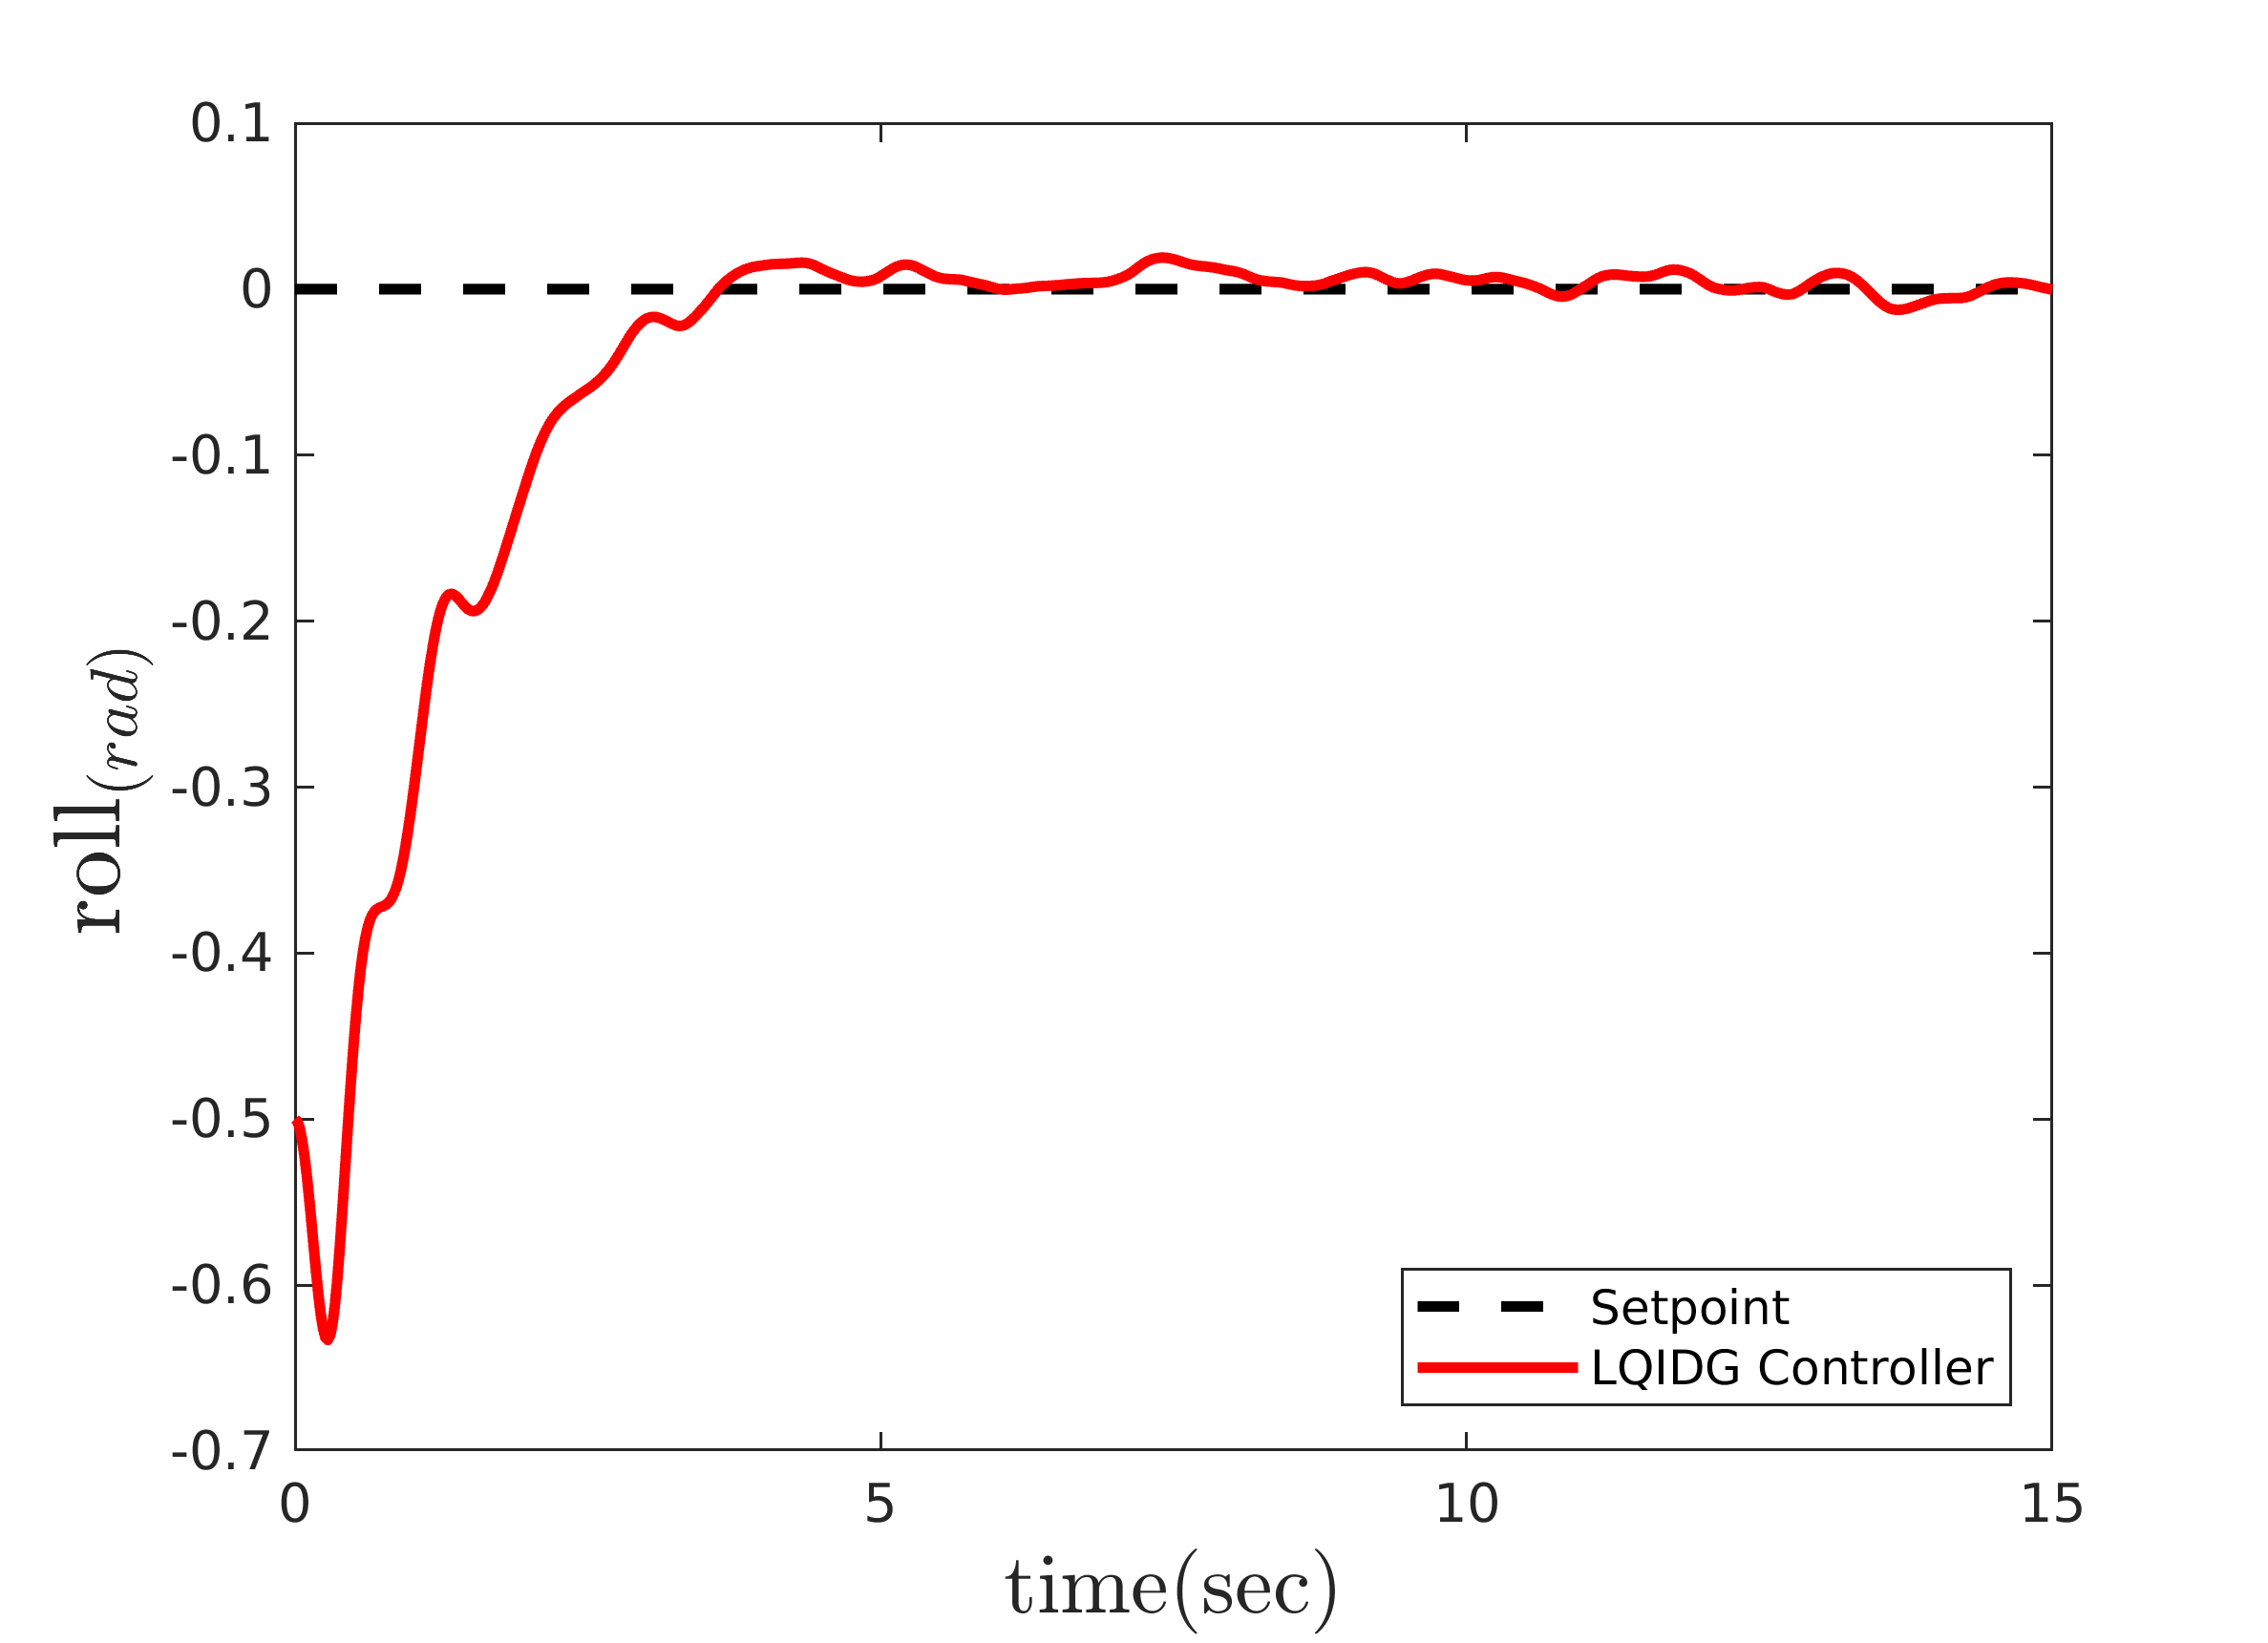
\includegraphics[width=12cm]{../Figures/MIL/LQIDG/3DOF/lqidg_roll.png}
%		\caption{تغییرات زاویه رول}
%	\end{subfigure}%
%	\begin{subfigure}
%		\centering
%		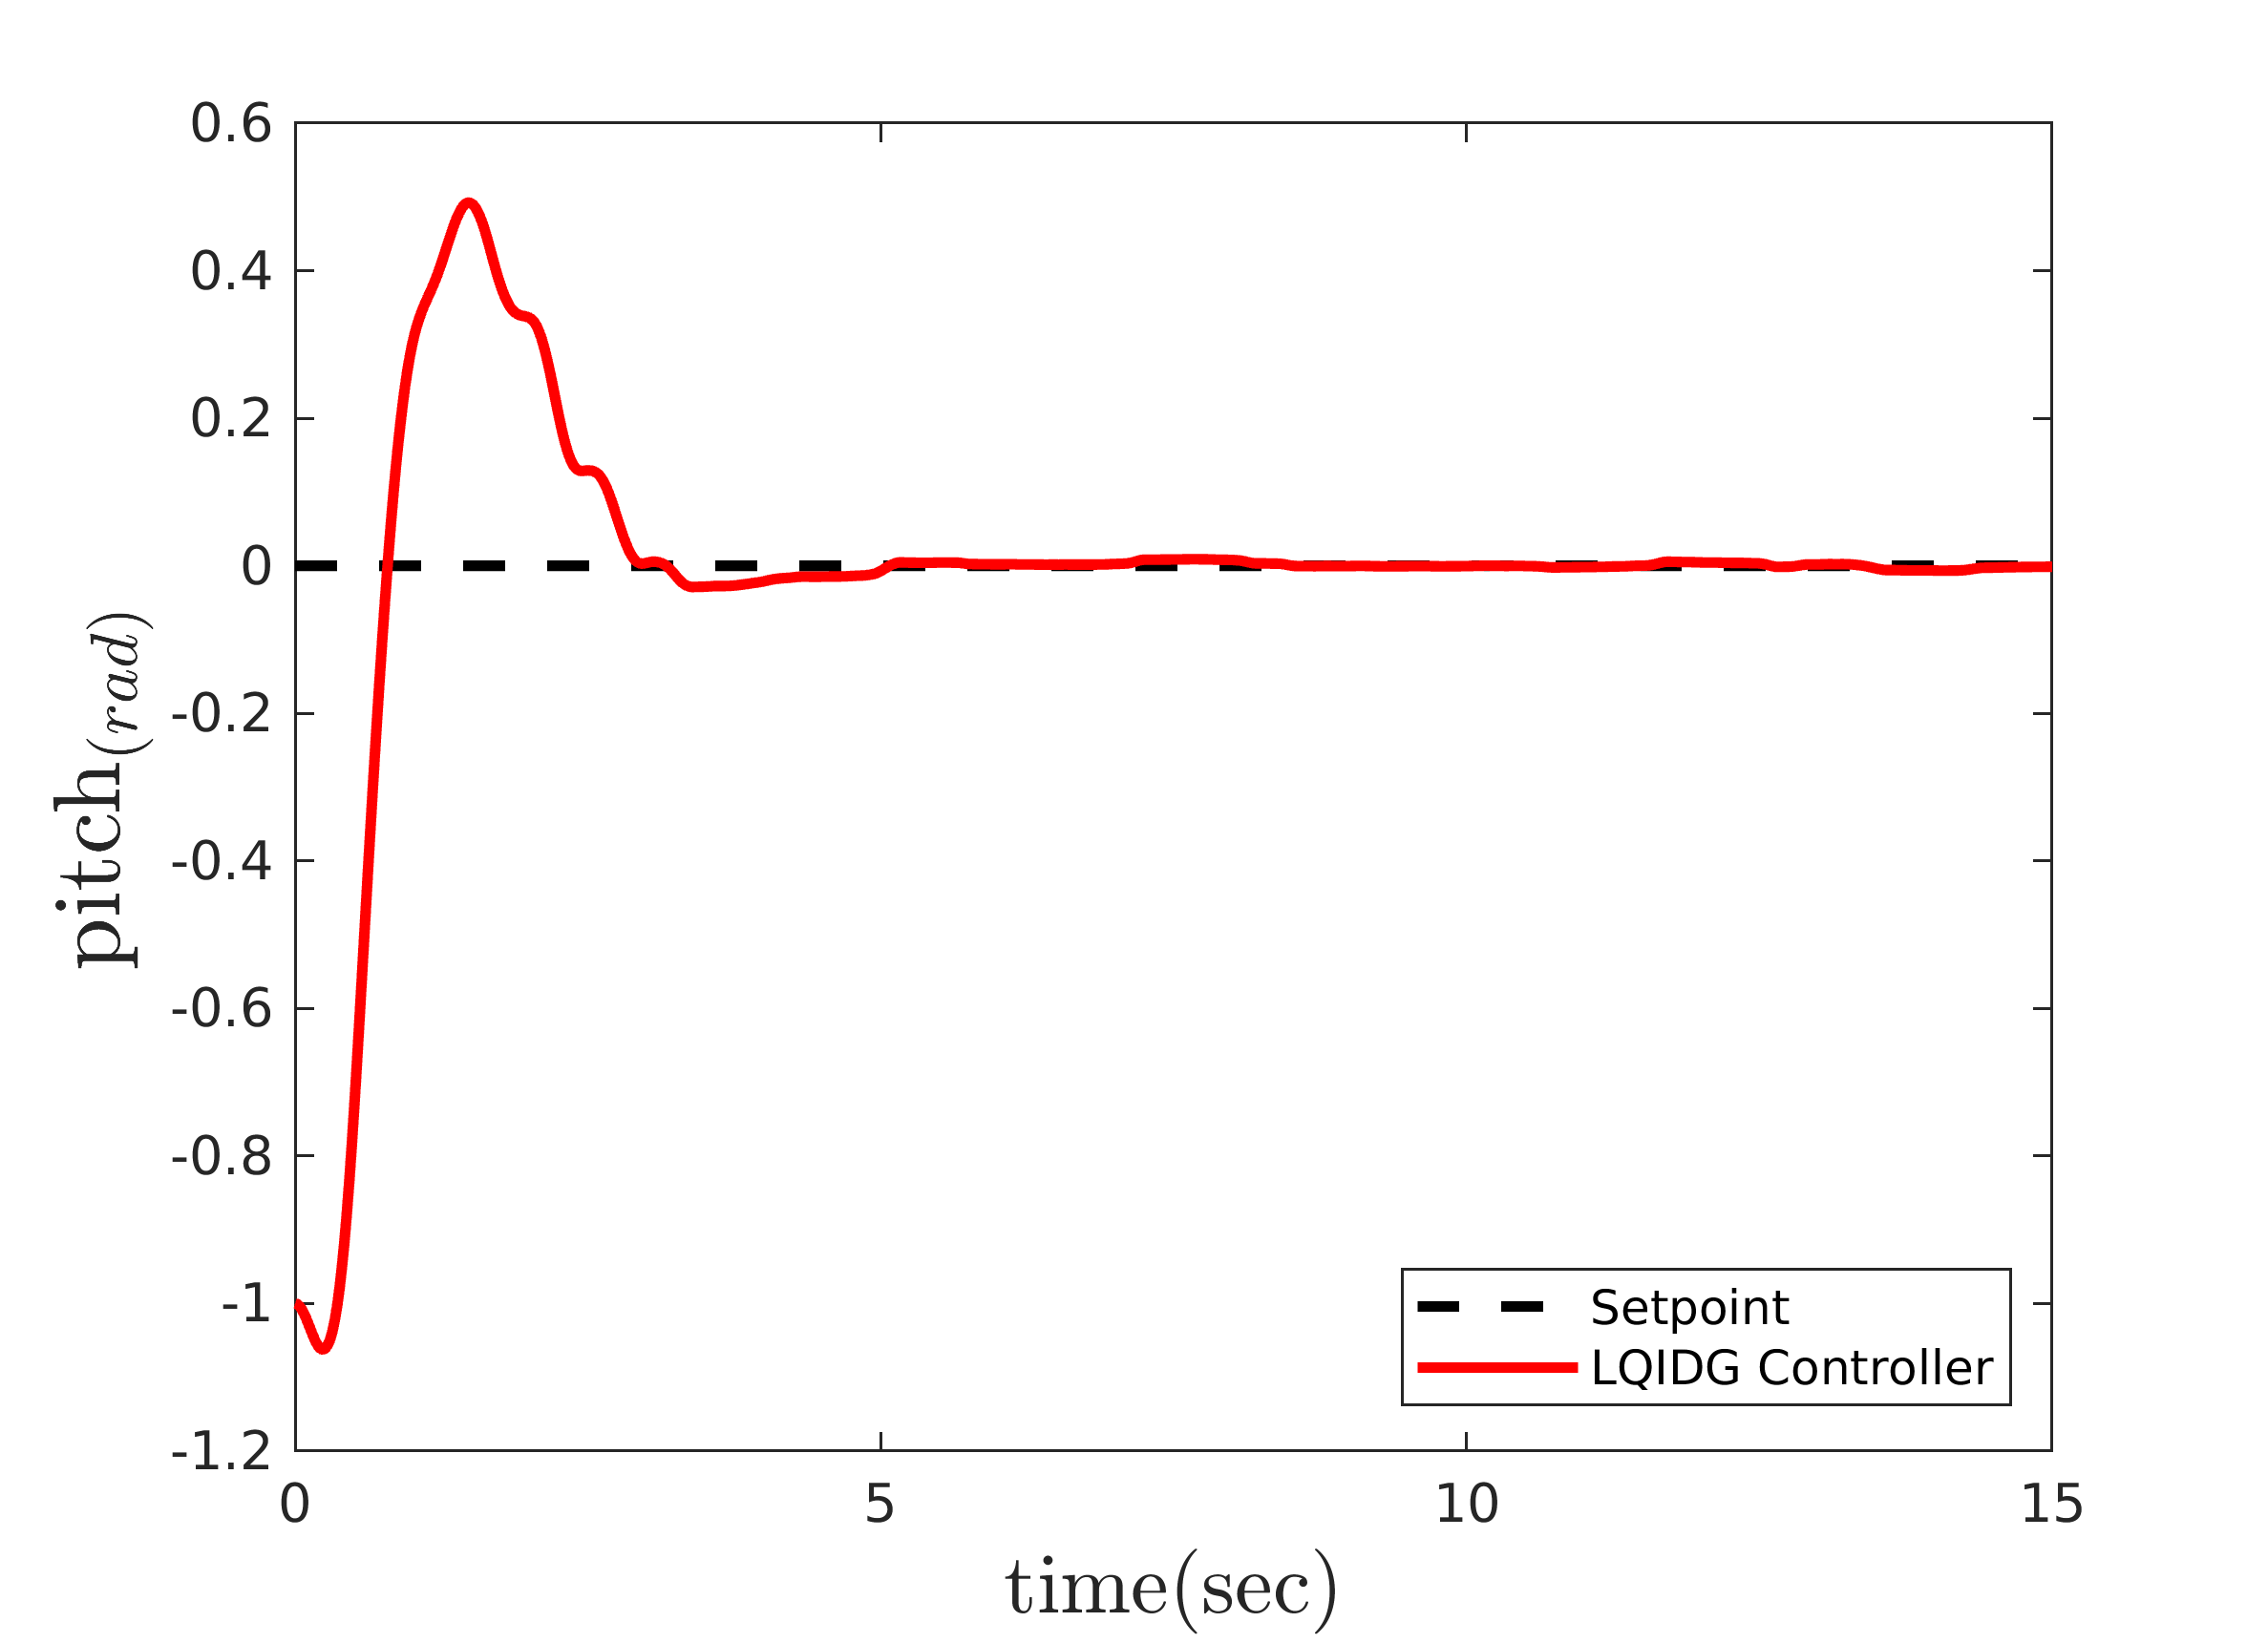
\includegraphics[width=12cm]{../Figures/MIL/LQIDG/3DOF/lqidg_pitch.png}
%		\caption{تغییرات زاویه پیچ}
%	\end{subfigure}
%	\caption{‫‪عملکرد کنترل‌کننده LQIDG در کنترل زاویه رول، پیچ و یاد (تعقیب ورودی صفر)}
%\end{figure}
%
%\begin{figure}[H]
%	\centering
%	\begin{subfigure}[H]
%		\centering
%		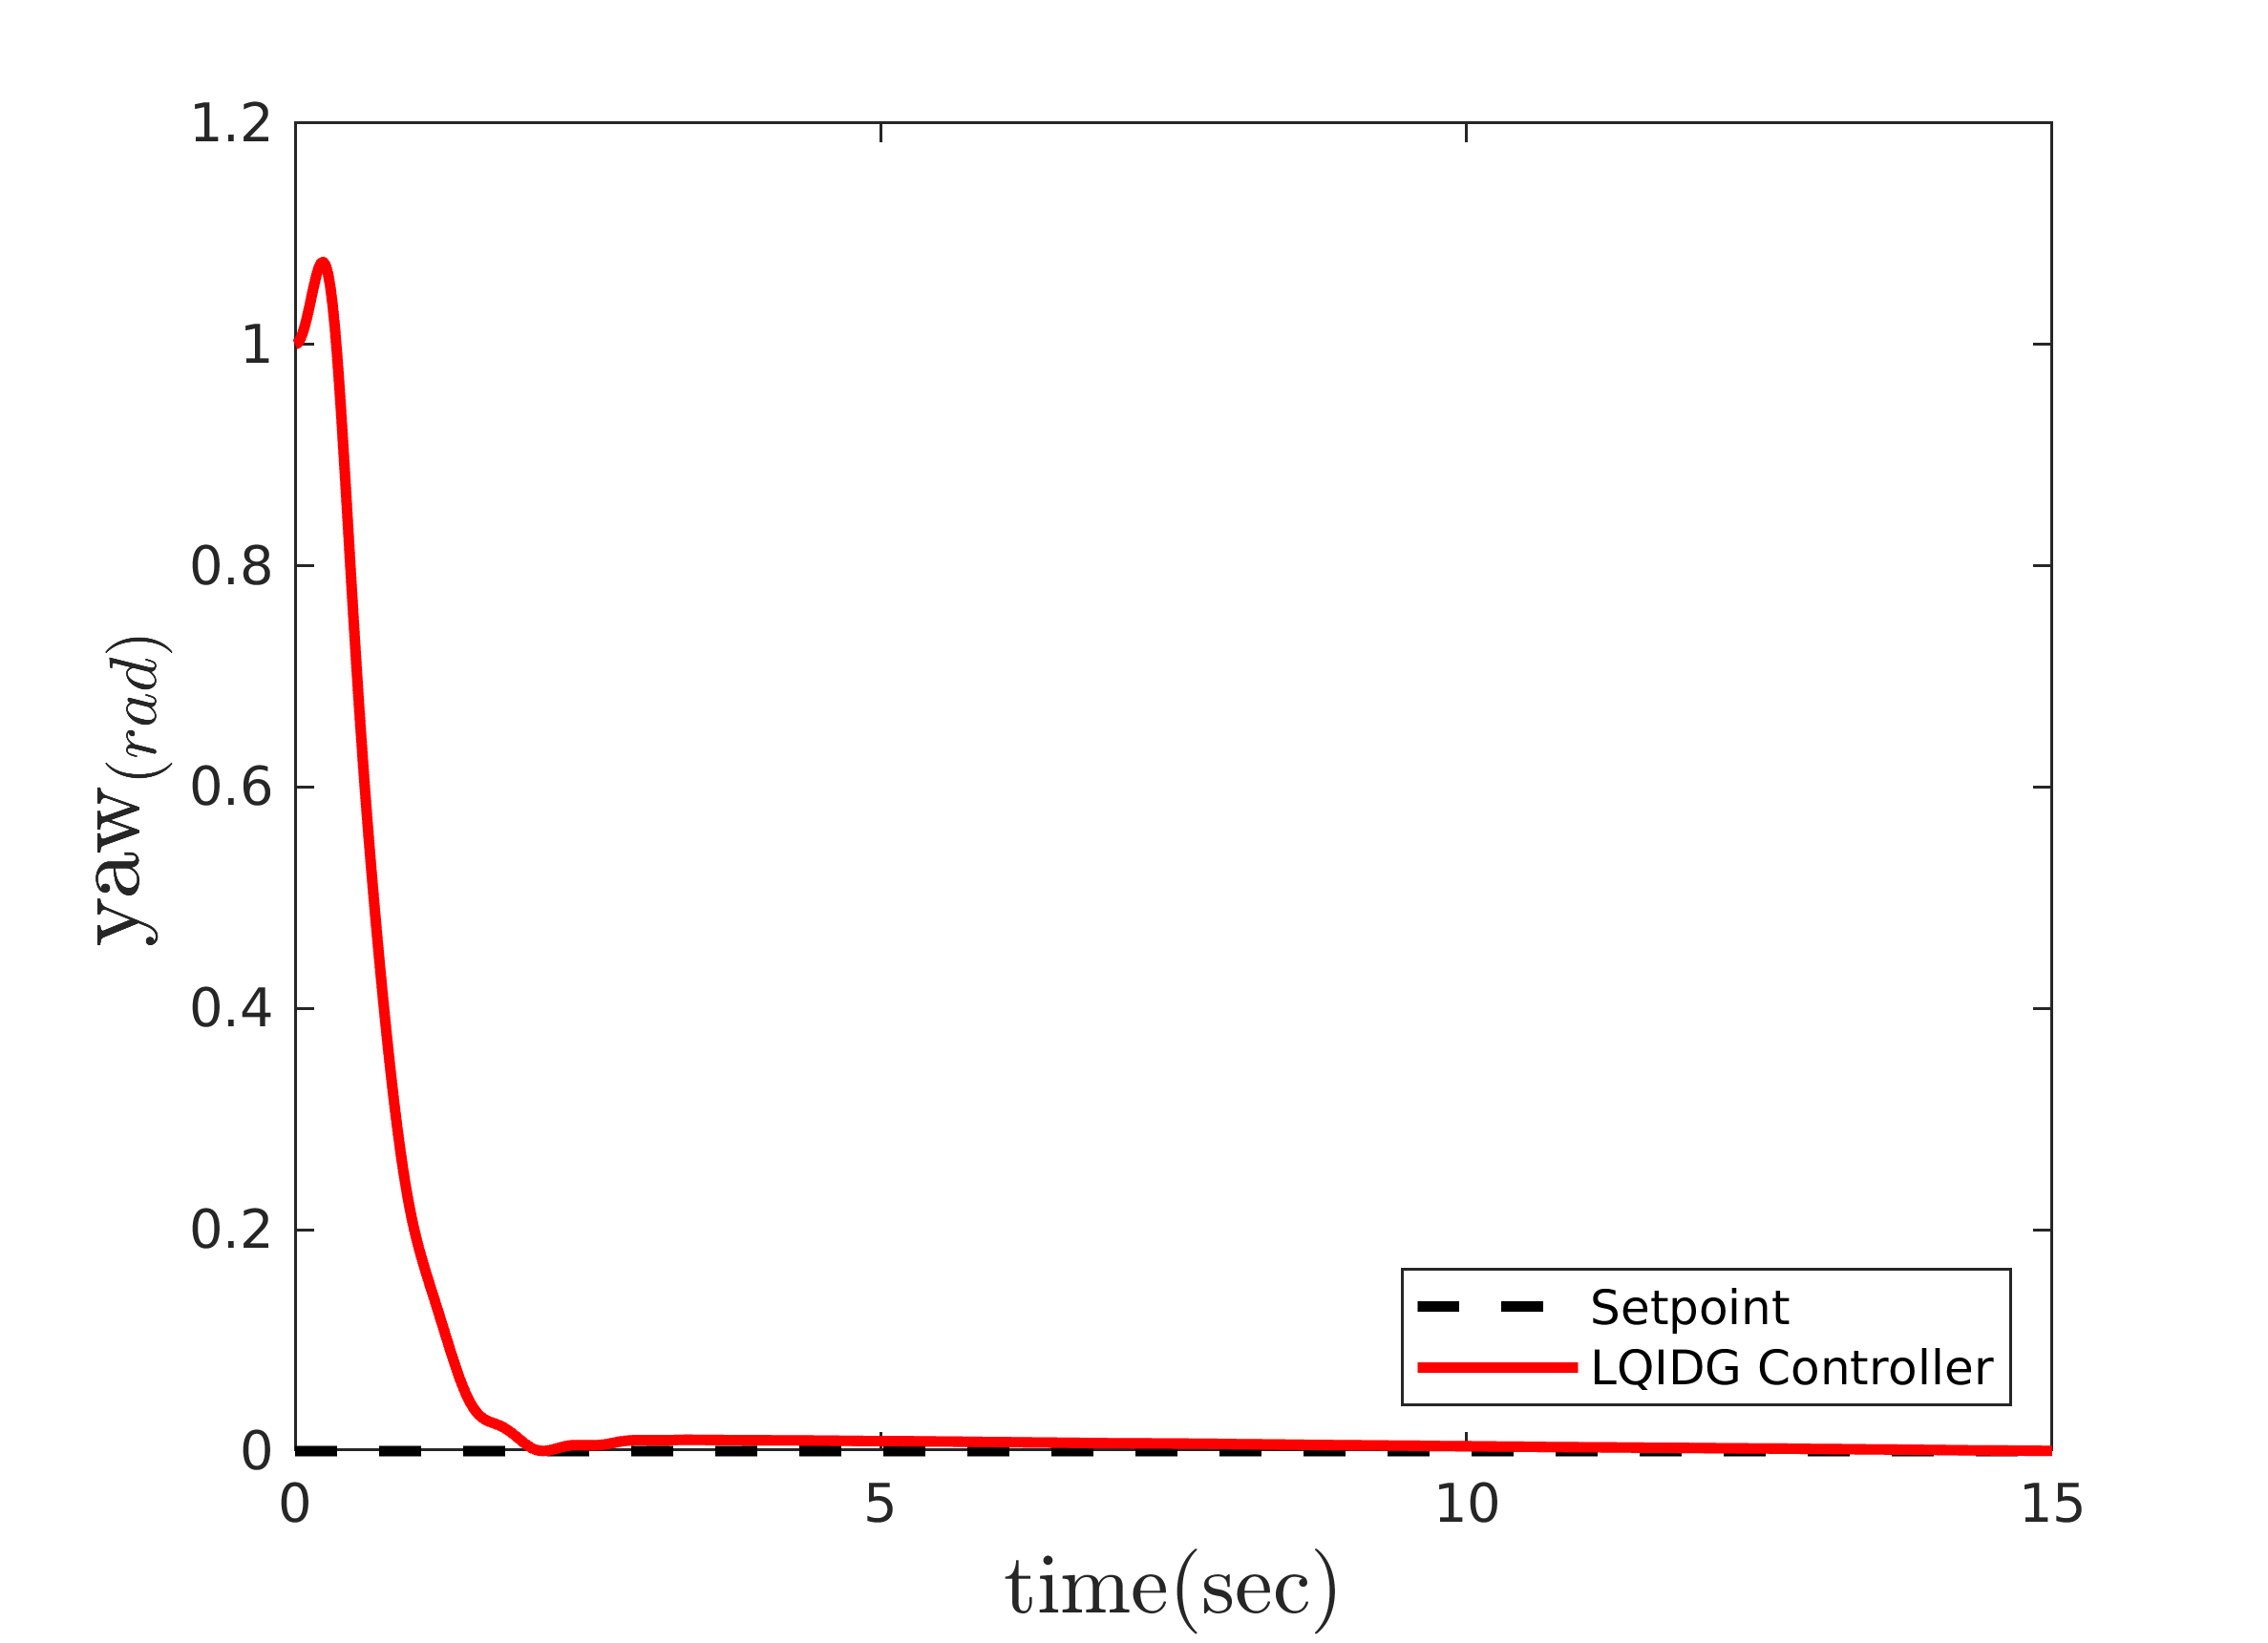
\includegraphics[width=12cm]{../Figures/MIL/LQIDG/3DOF/lqidg_yaw.png}
%		\caption{تغییرات زاویه یاو}
%	\end{subfigure}
%	\caption{‫‪عملکرد کنترل‌کننده LQIDG در کنترل زاویه رول، پیچ و یاد (تعقیب ورودی صفر)}
%\end{figure}
\begin{figure}[H]
	\centering
\subfigure[تغییرات زاویه رول]{
	\centering
	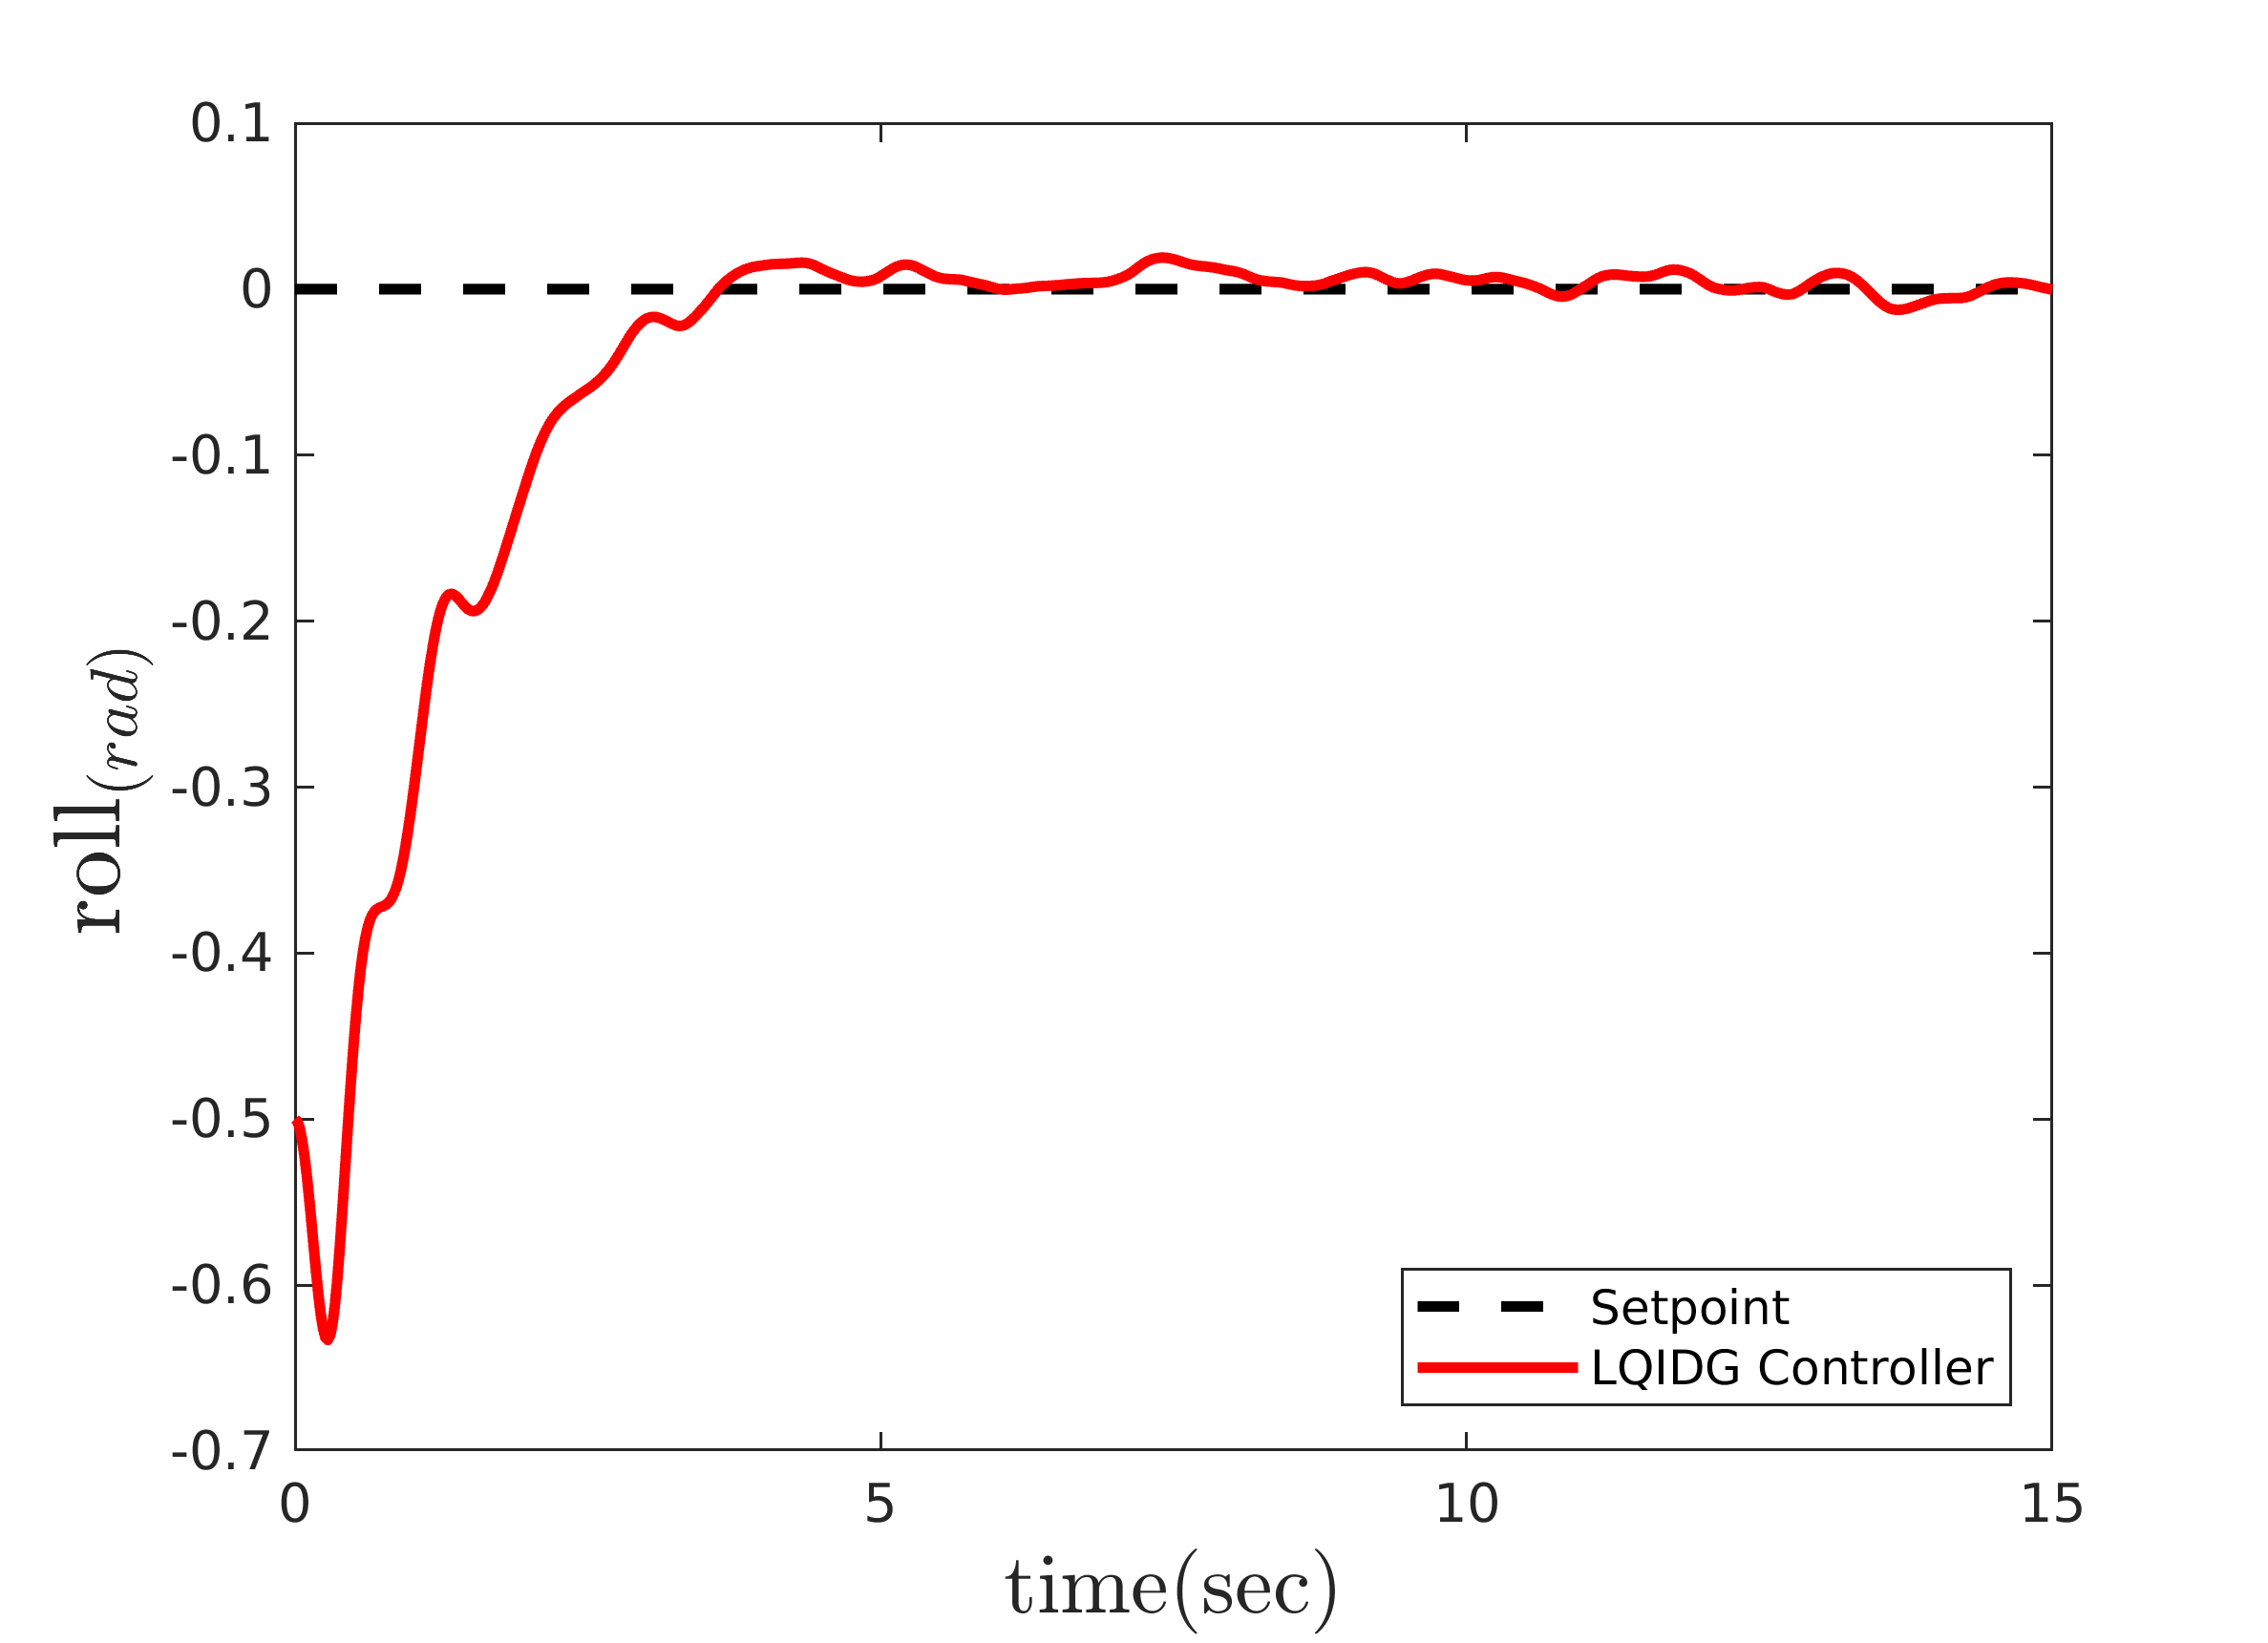
\includegraphics[width=.6\linewidth]{../Figures/MIL/LQIDG/3DOF/lqidg_roll.png}
}
\subfigure[تغییرات زاویه پیچ]{
	\centering
	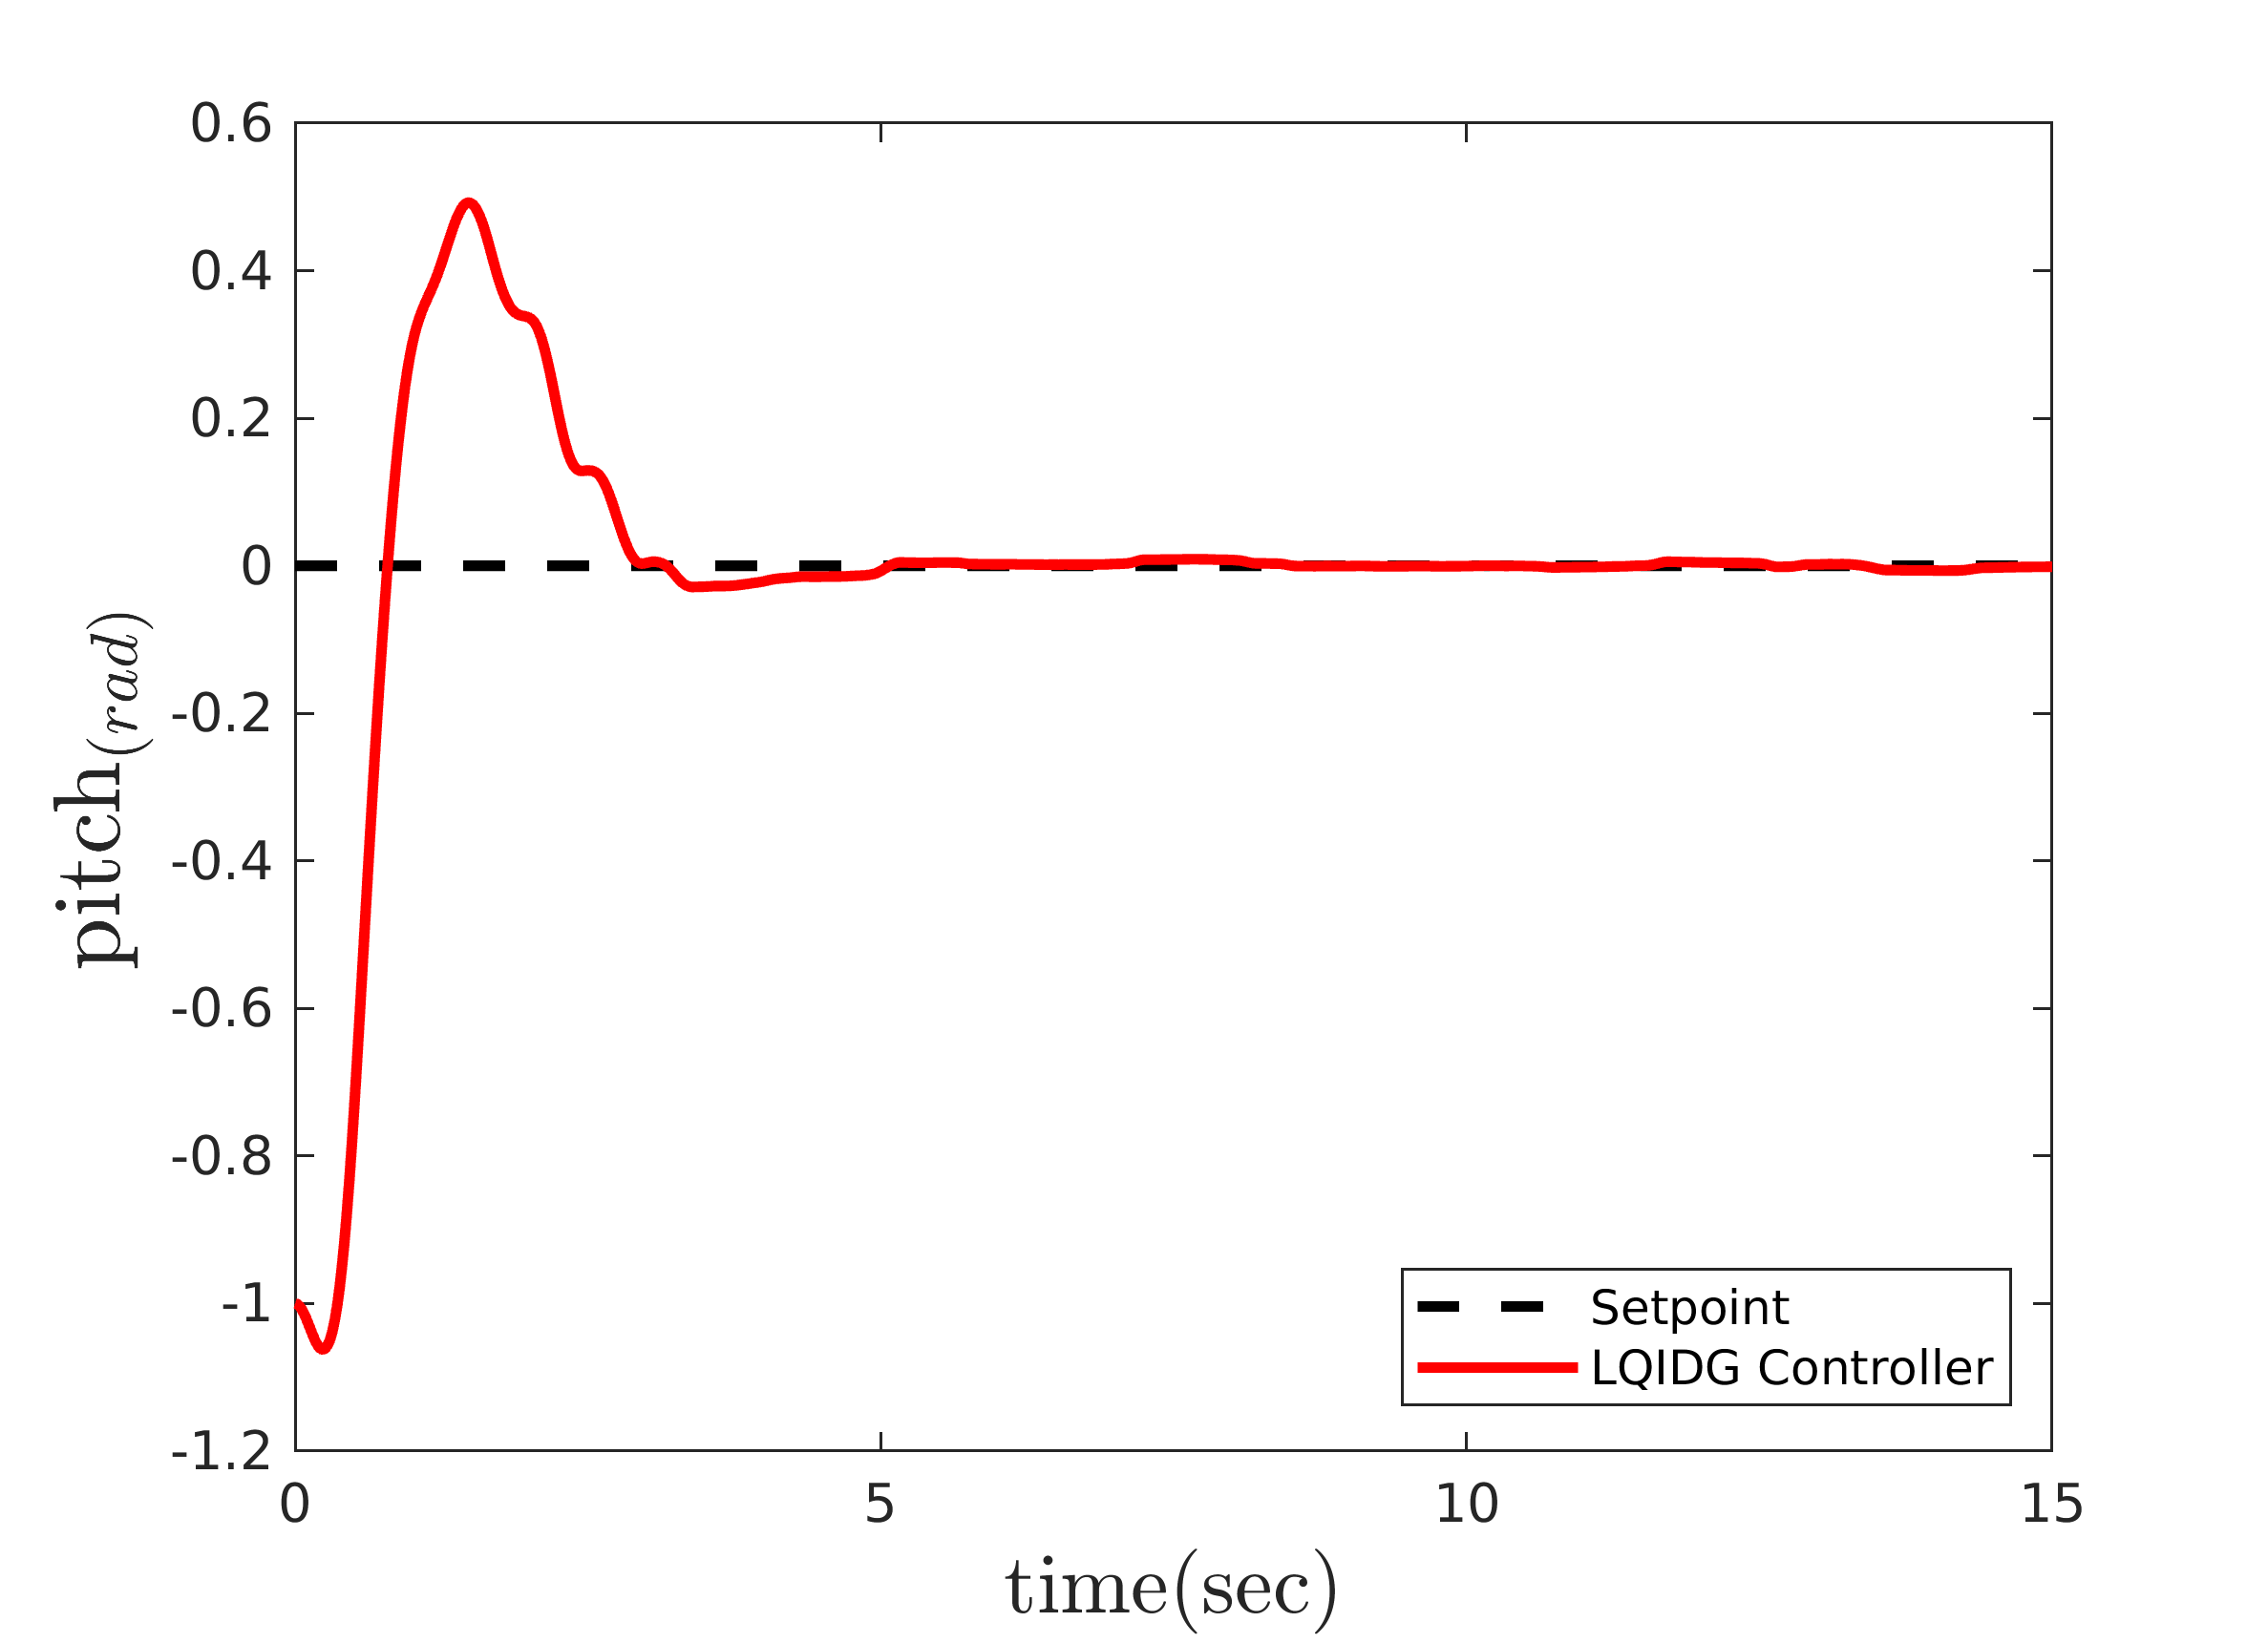
\includegraphics[width=.6\linewidth]{../Figures/MIL/LQIDG/3DOF/lqidg_pitch.png}
}
\subfigure[تغییرات زاویه یاو]{
	\centering
	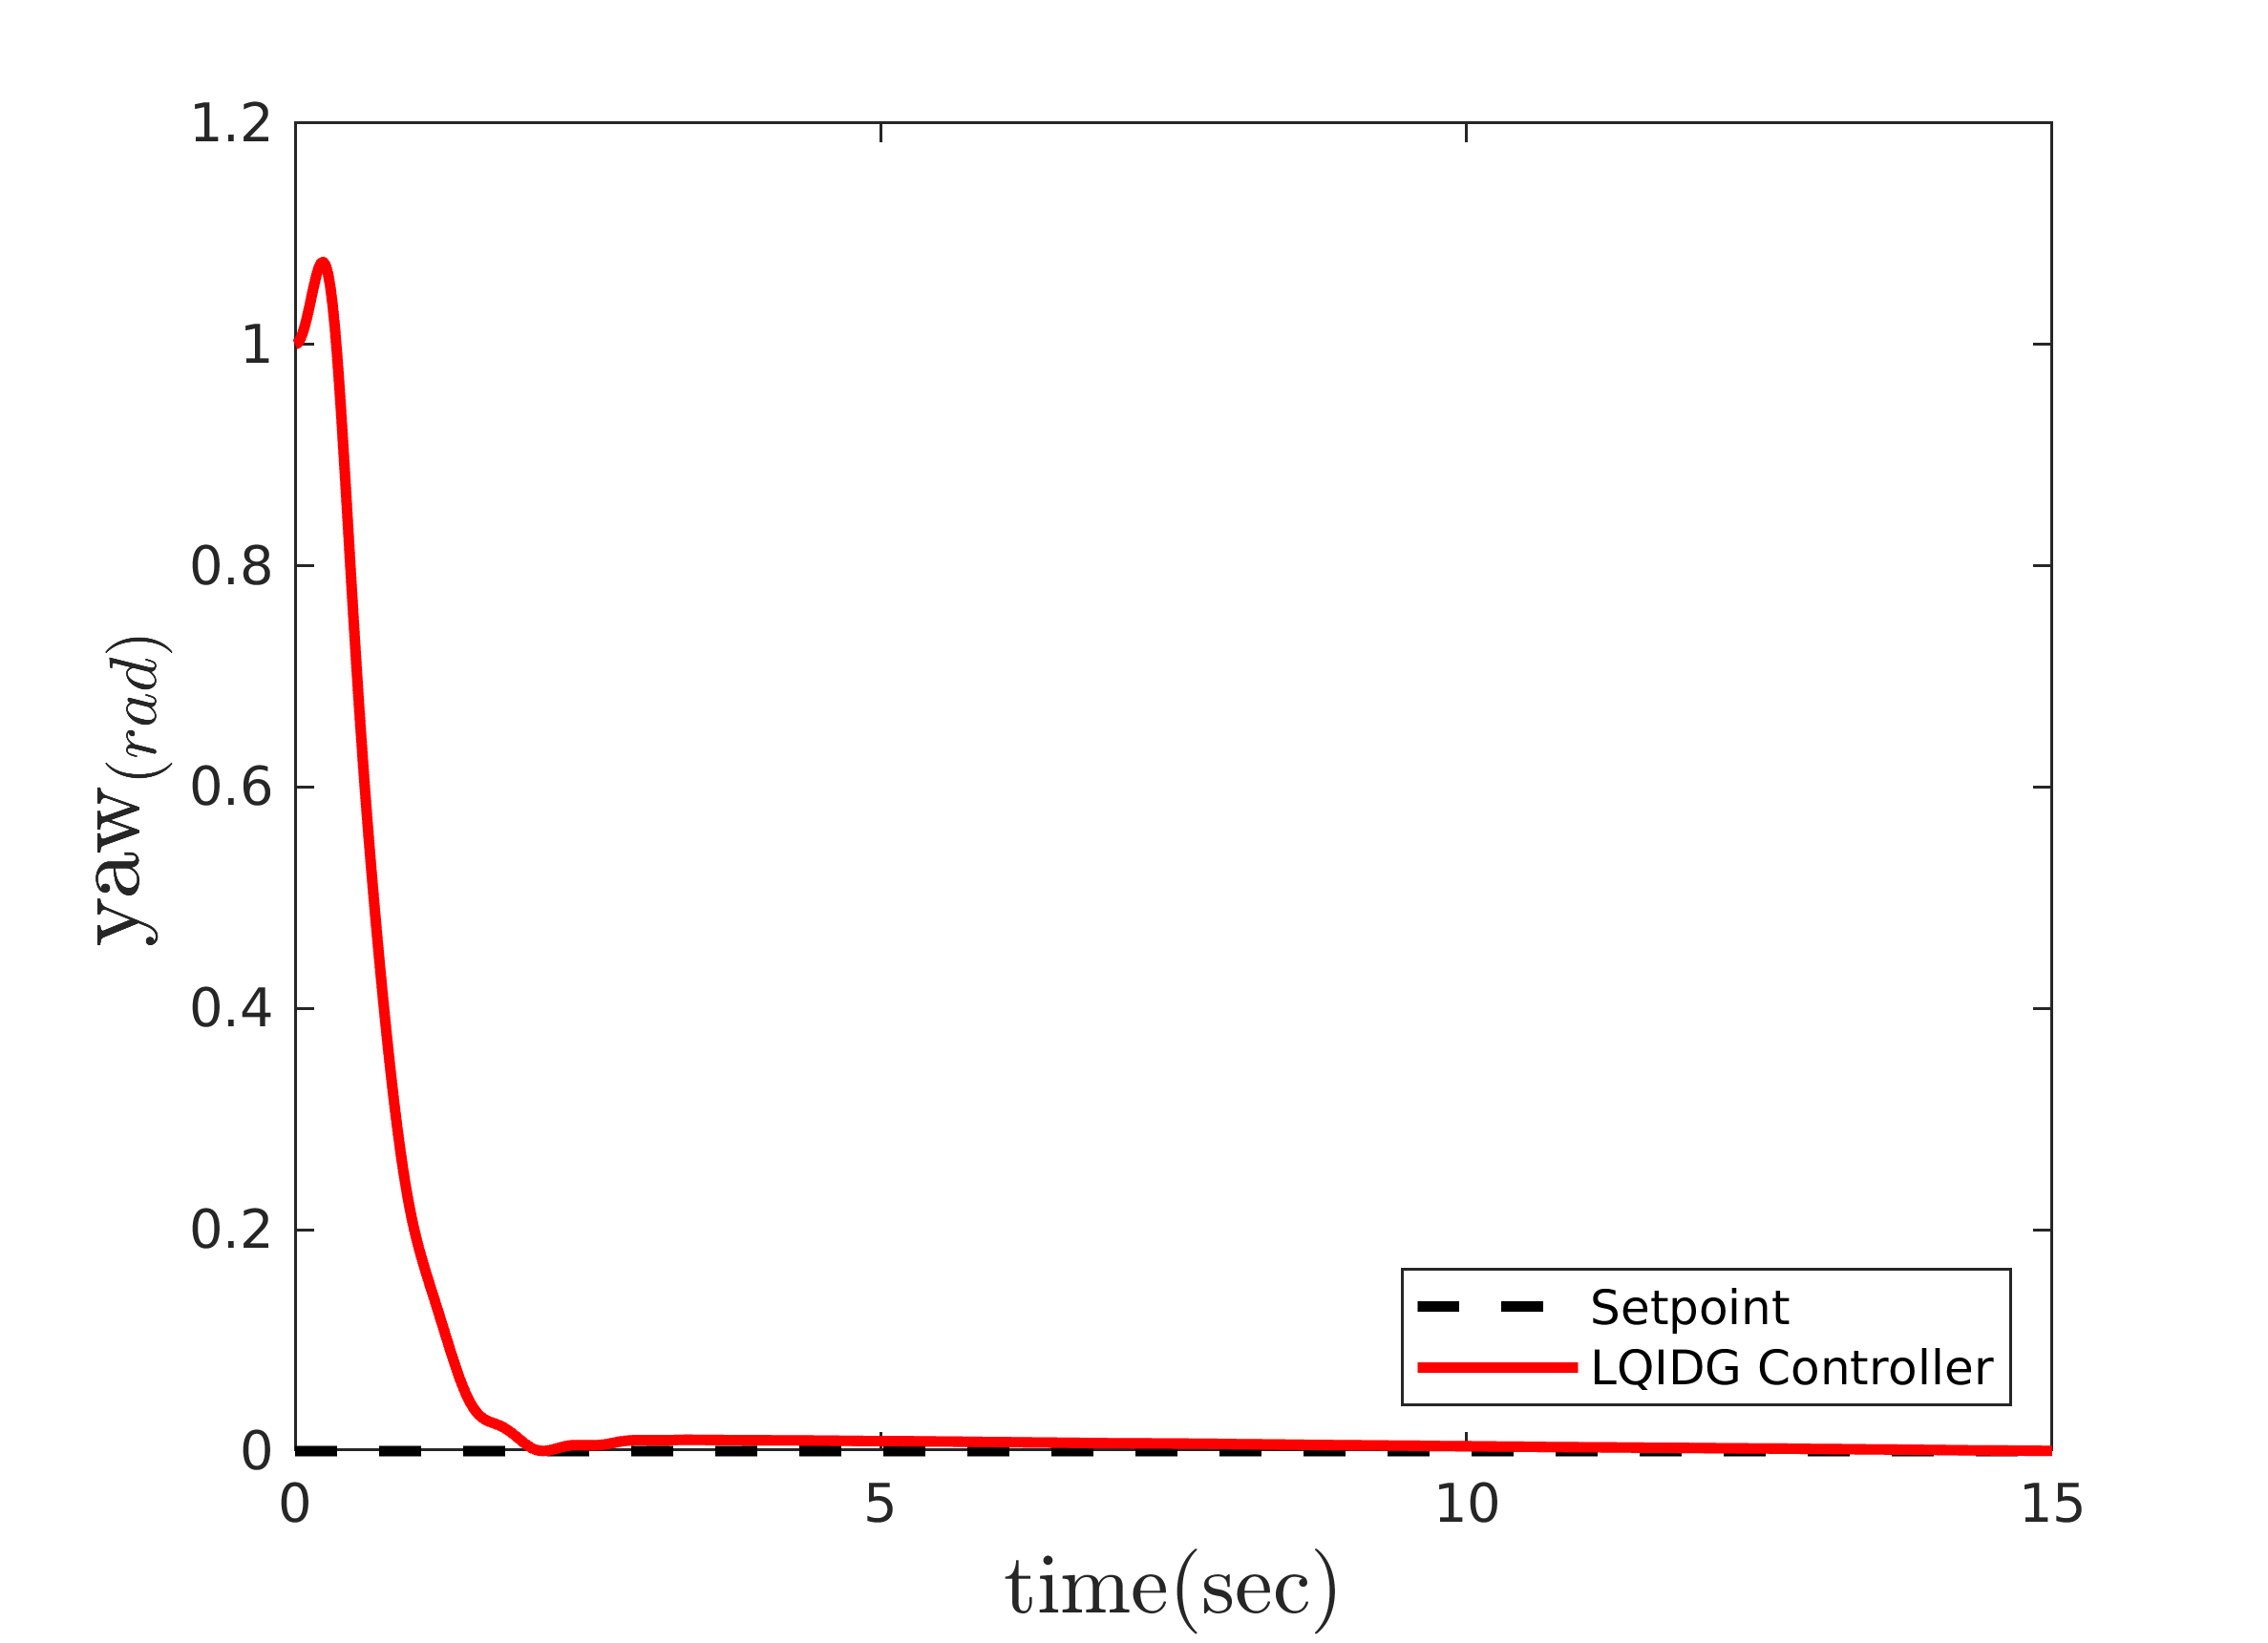
\includegraphics[width=.6\linewidth]{../Figures/MIL/LQIDG/3DOF/lqidg_yaw.png}
}
	\caption{‫‪عملکرد کنترل‌کننده LQIDG در کنترل زاویه رول، پیچ و یاد (تعقیب ورودی صفر)}
\end{figure}


\begin{figure}[H]
	\centering
	\subfigure[موتور شماره یک]{
		\centering
		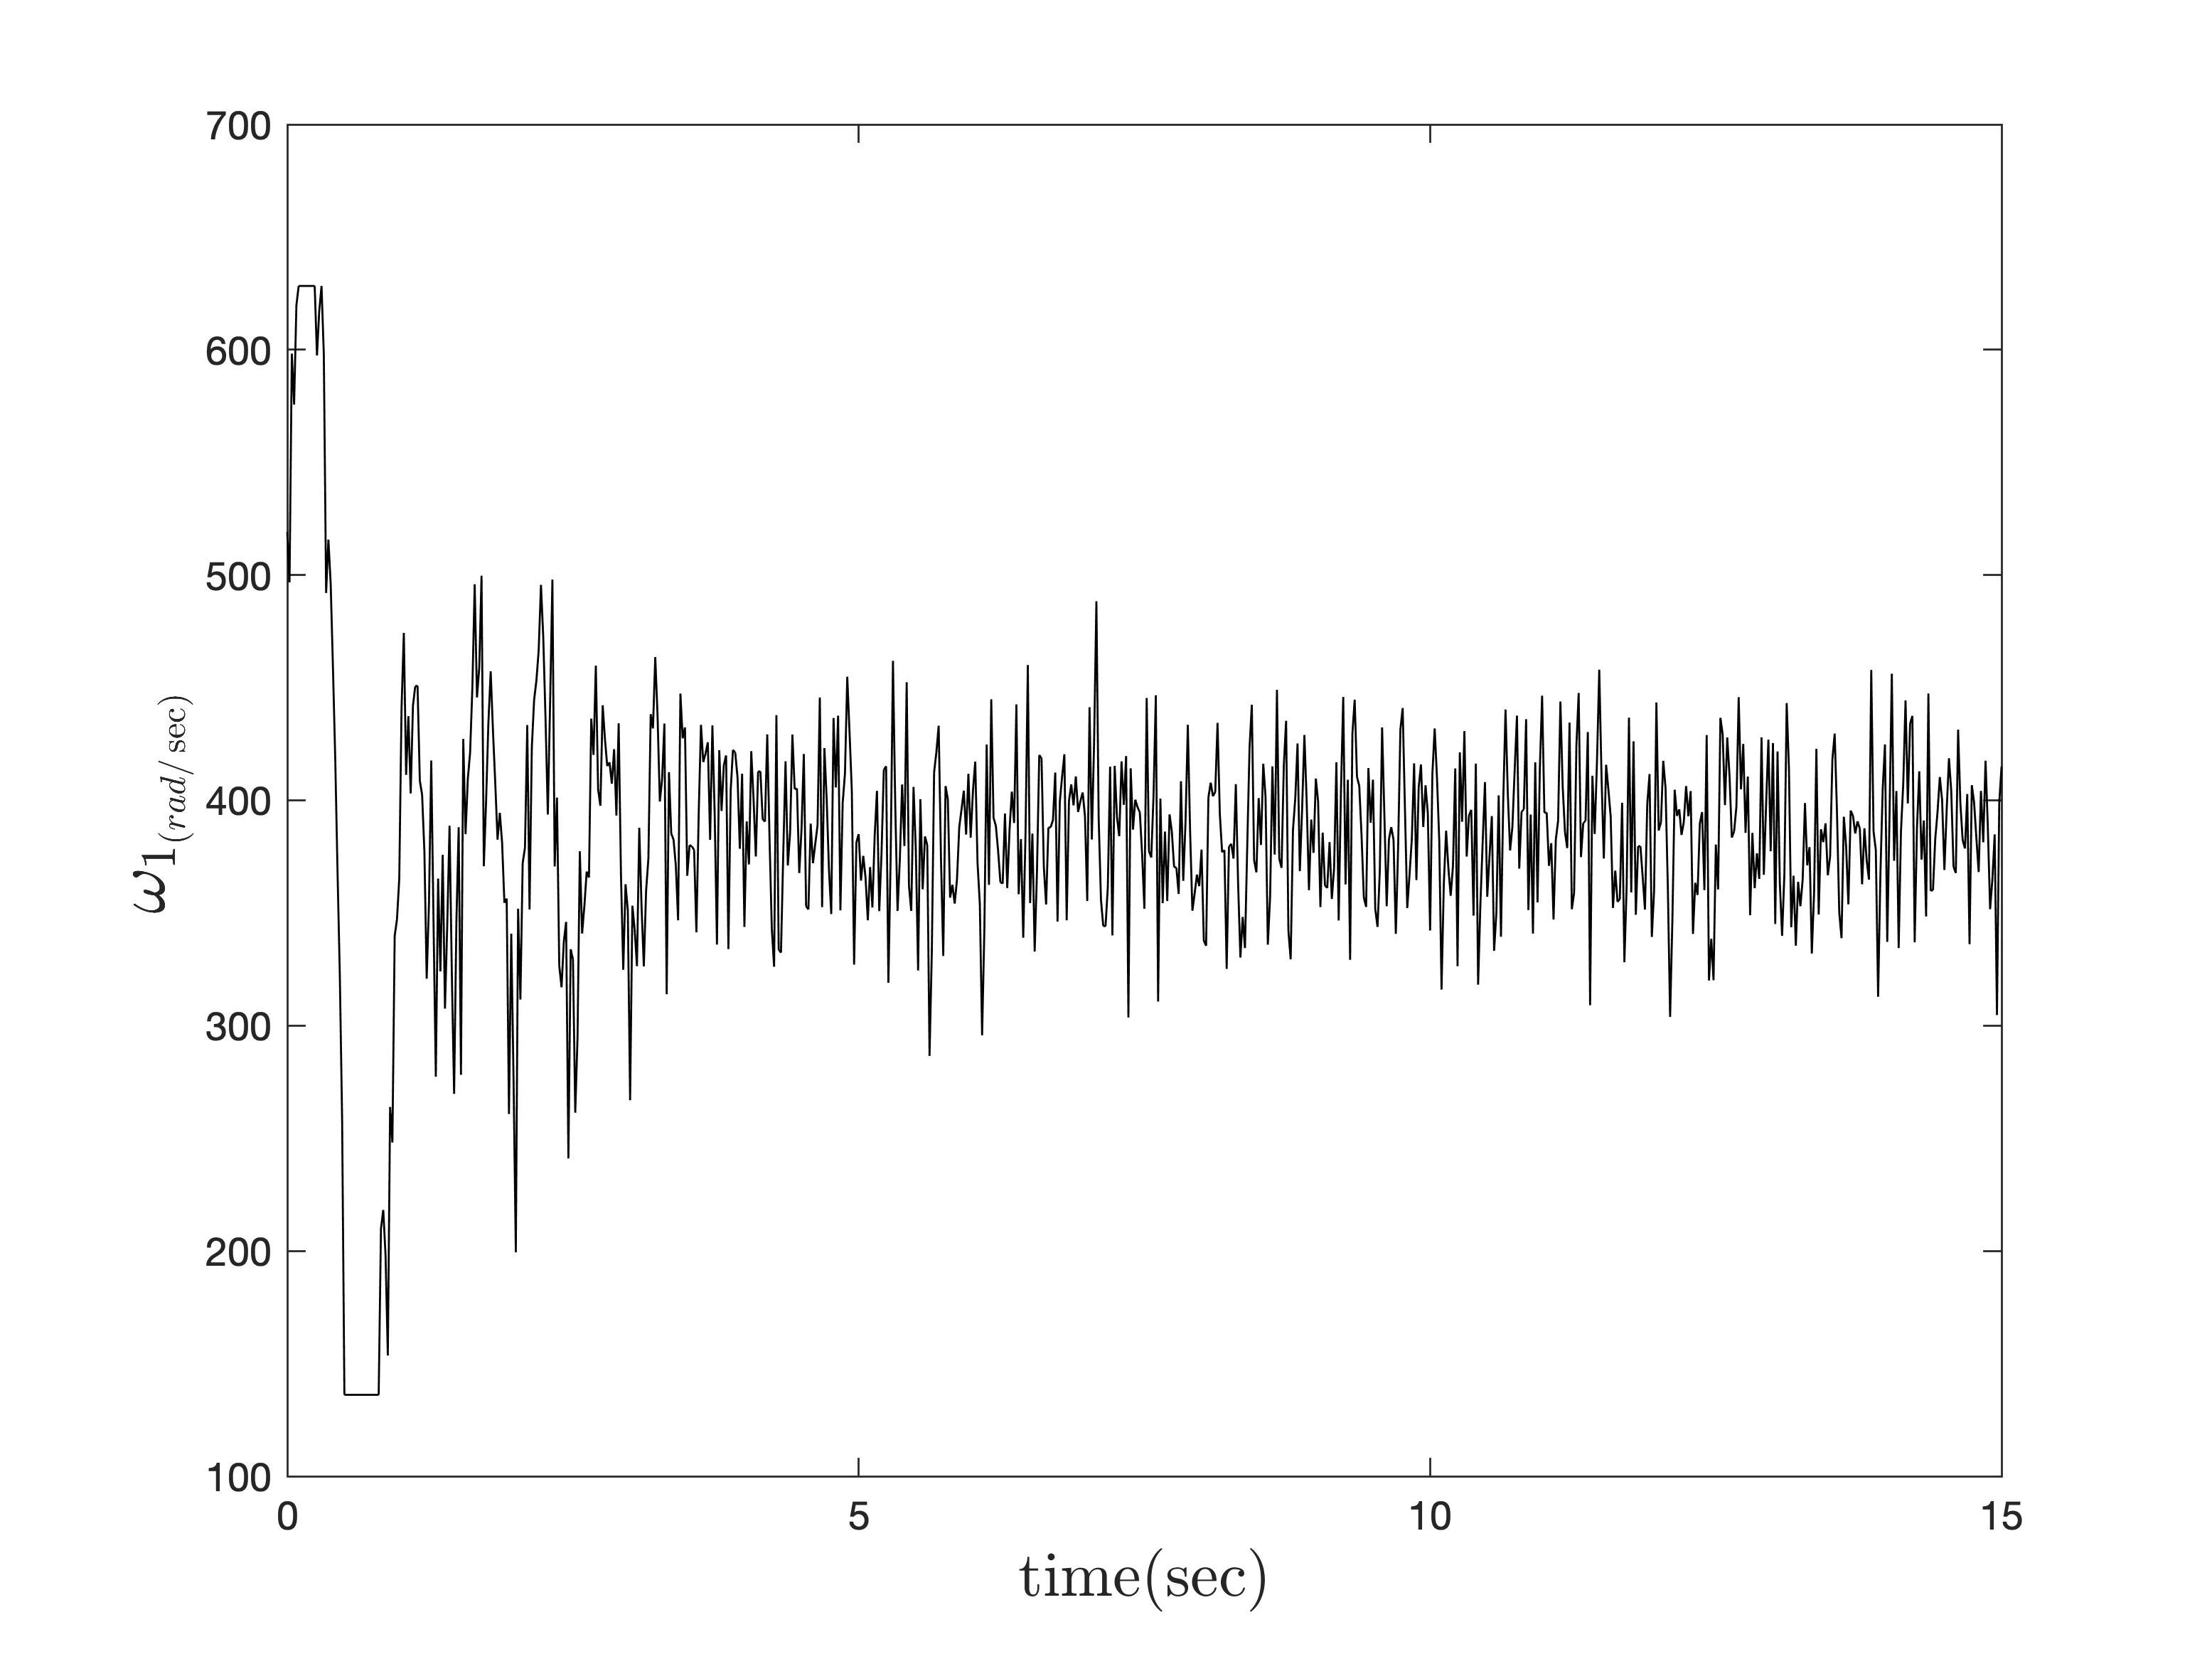
\includegraphics[width=.45\linewidth]{../Figures/MIL/LQIDG/3DOF/lqidg_roll_pitch_Omega_1.png}
	}
	\subfigure[موتور شماره دو]{
		\centering
		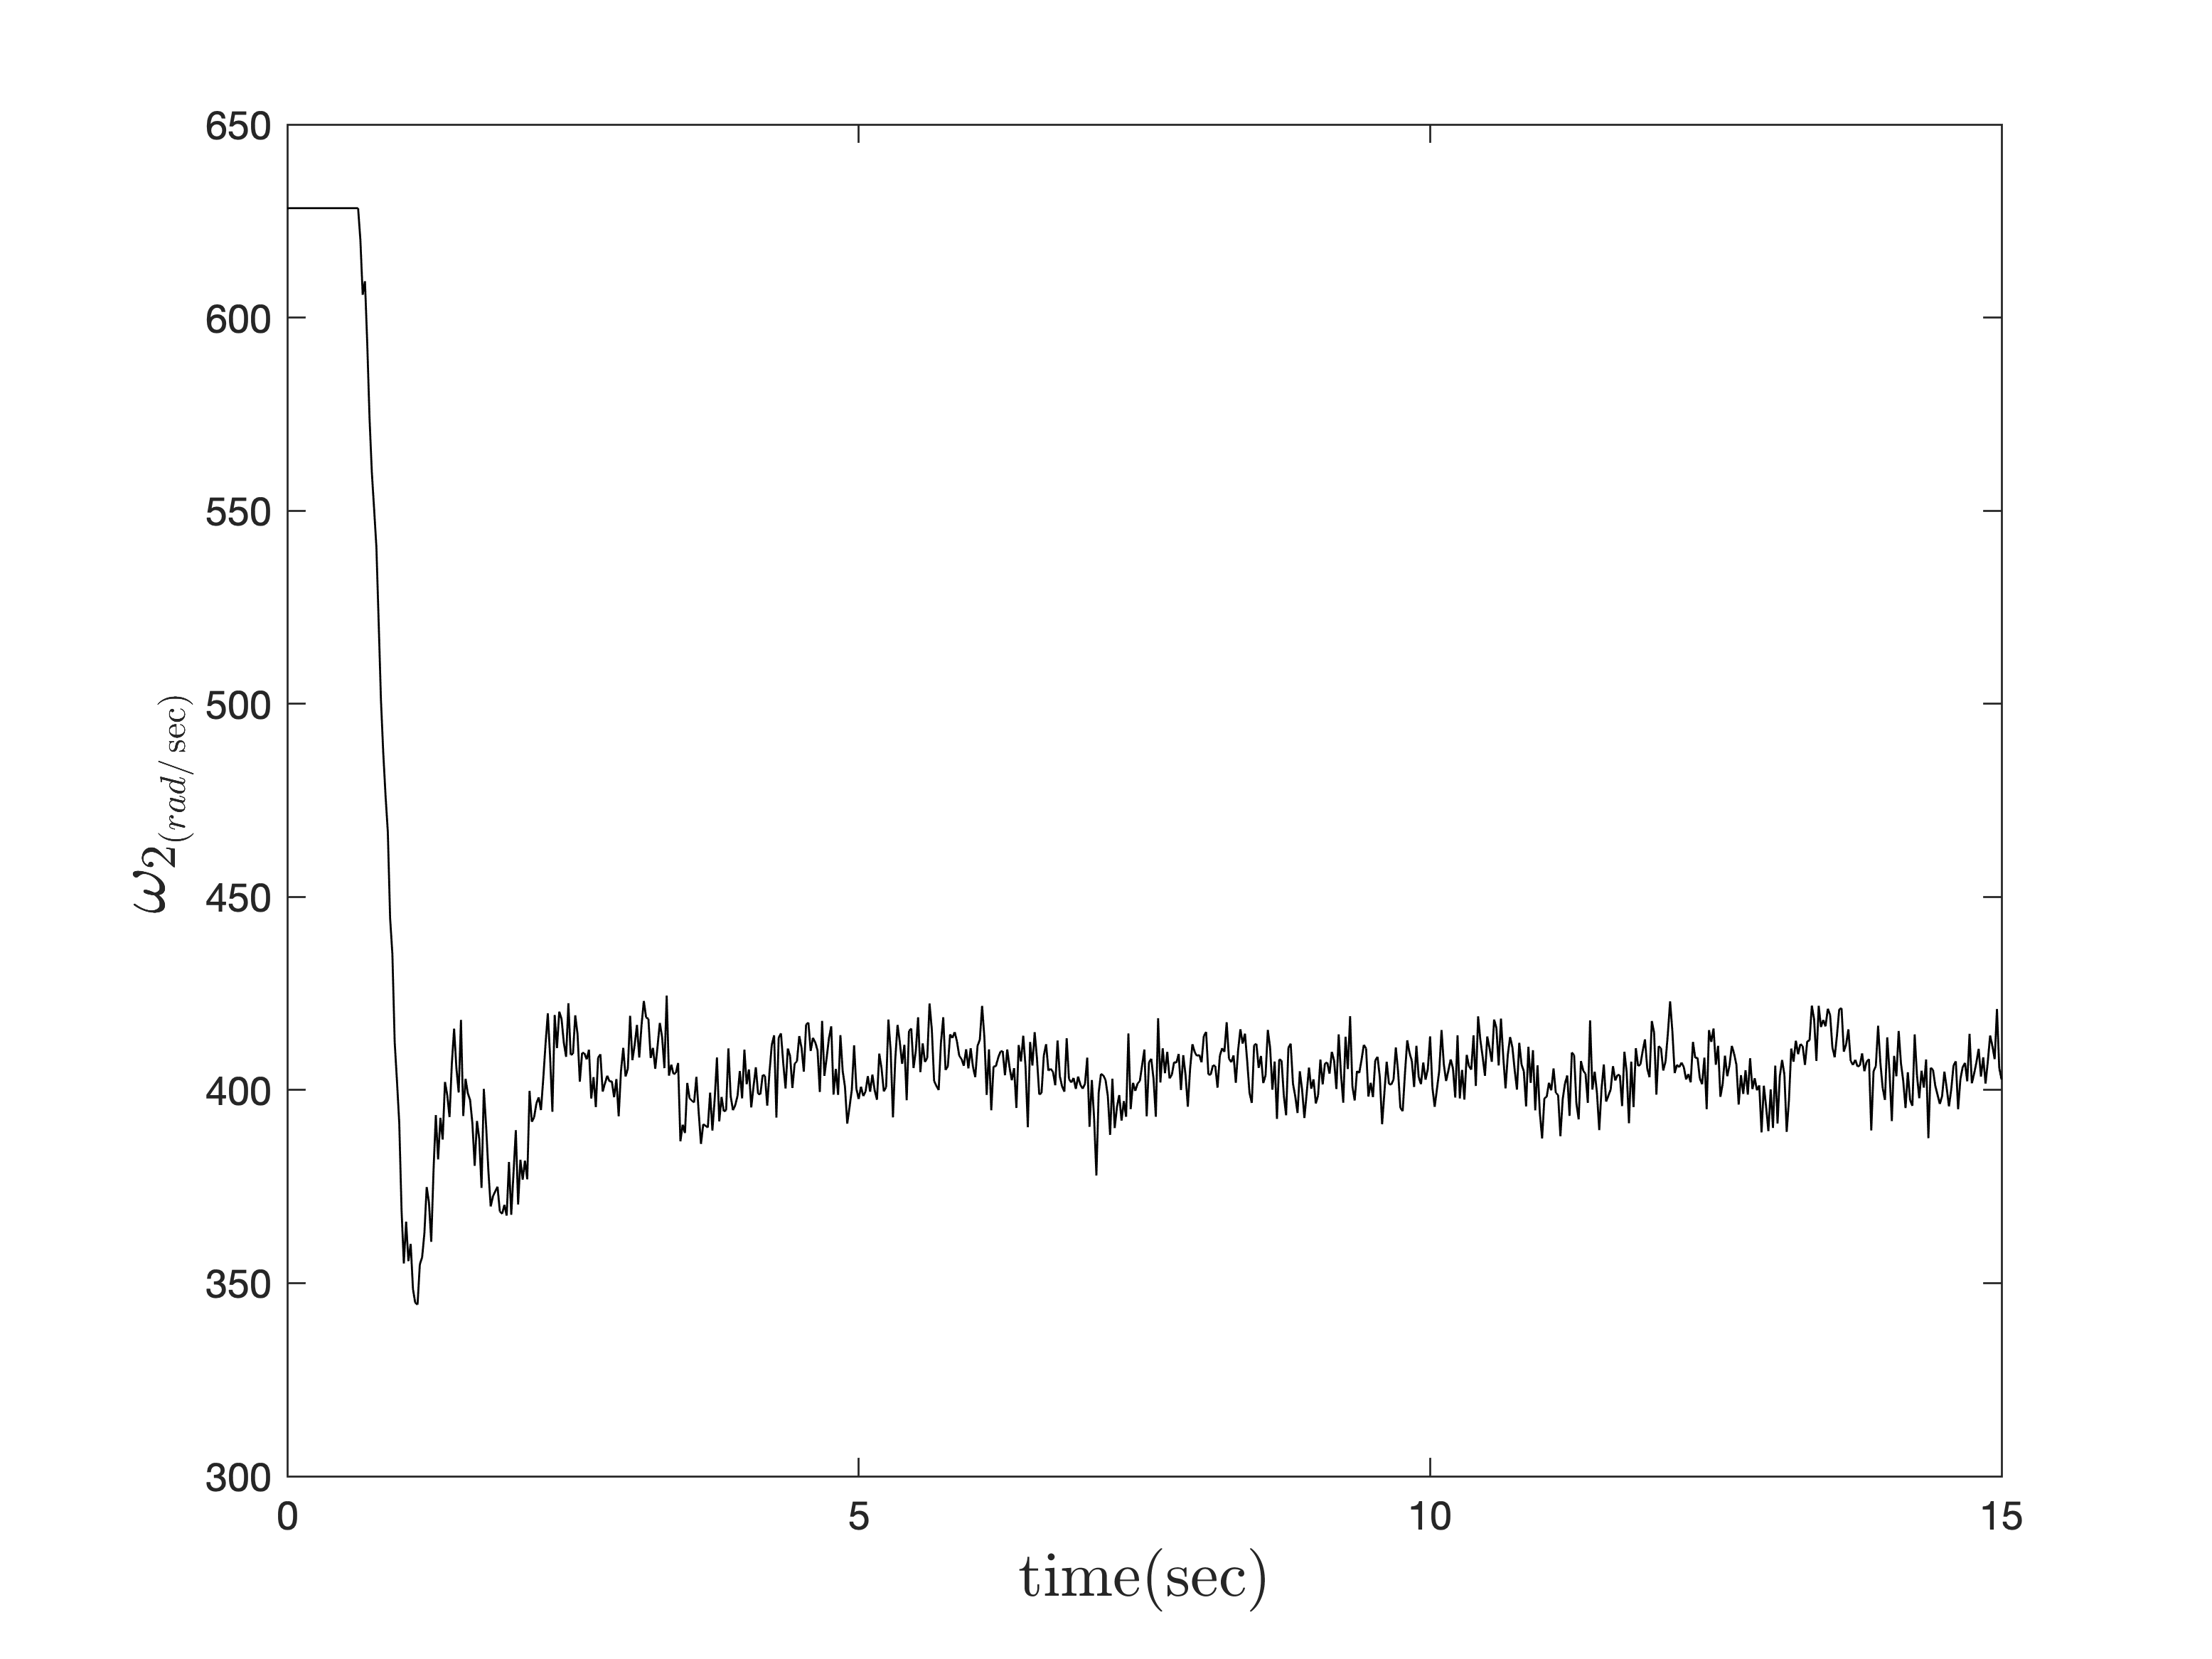
\includegraphics[width=.45\linewidth]{../Figures/MIL/LQIDG/3DOF/lqidg_roll_pitch_Omega_2.png}
	}
	\subfigure[موتور شماره سه]{
		\centering
		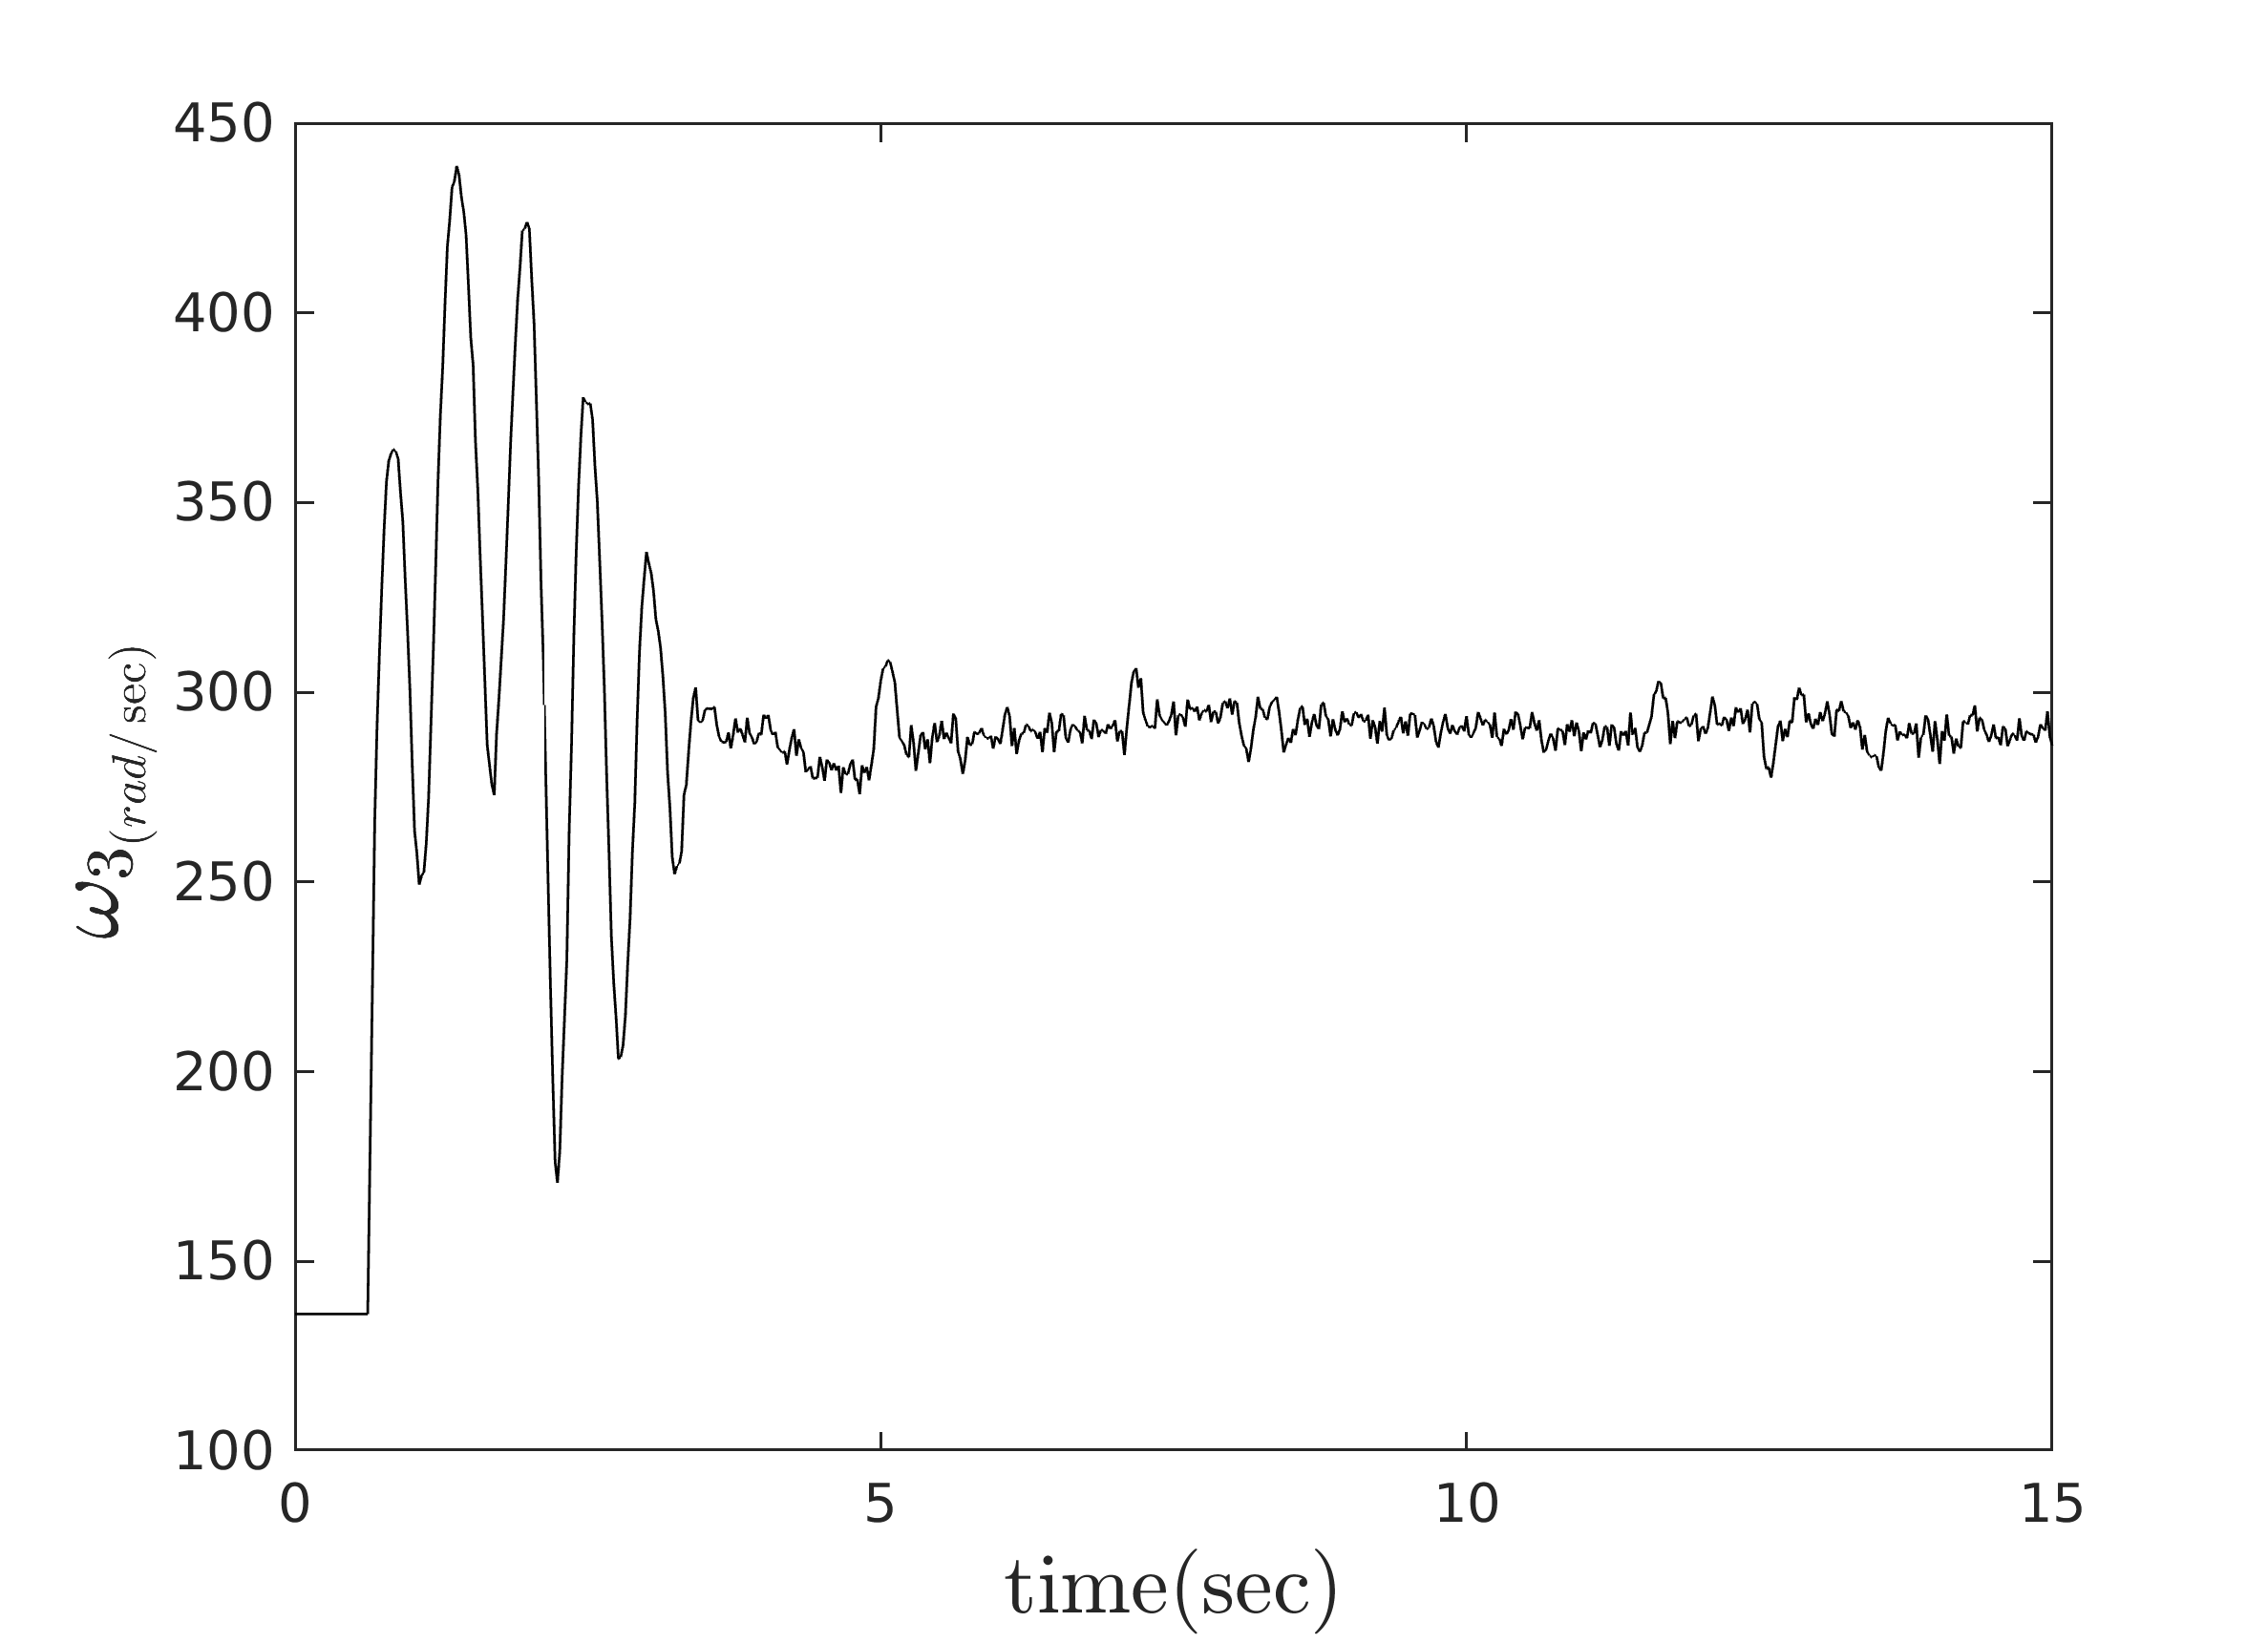
\includegraphics[width=.45\linewidth]{../Figures/MIL/LQIDG/3DOF/lqidg_roll_pitch_Omega_3.png}
	}
	\subfigure[موتور شماره چهار]{
		\centering
		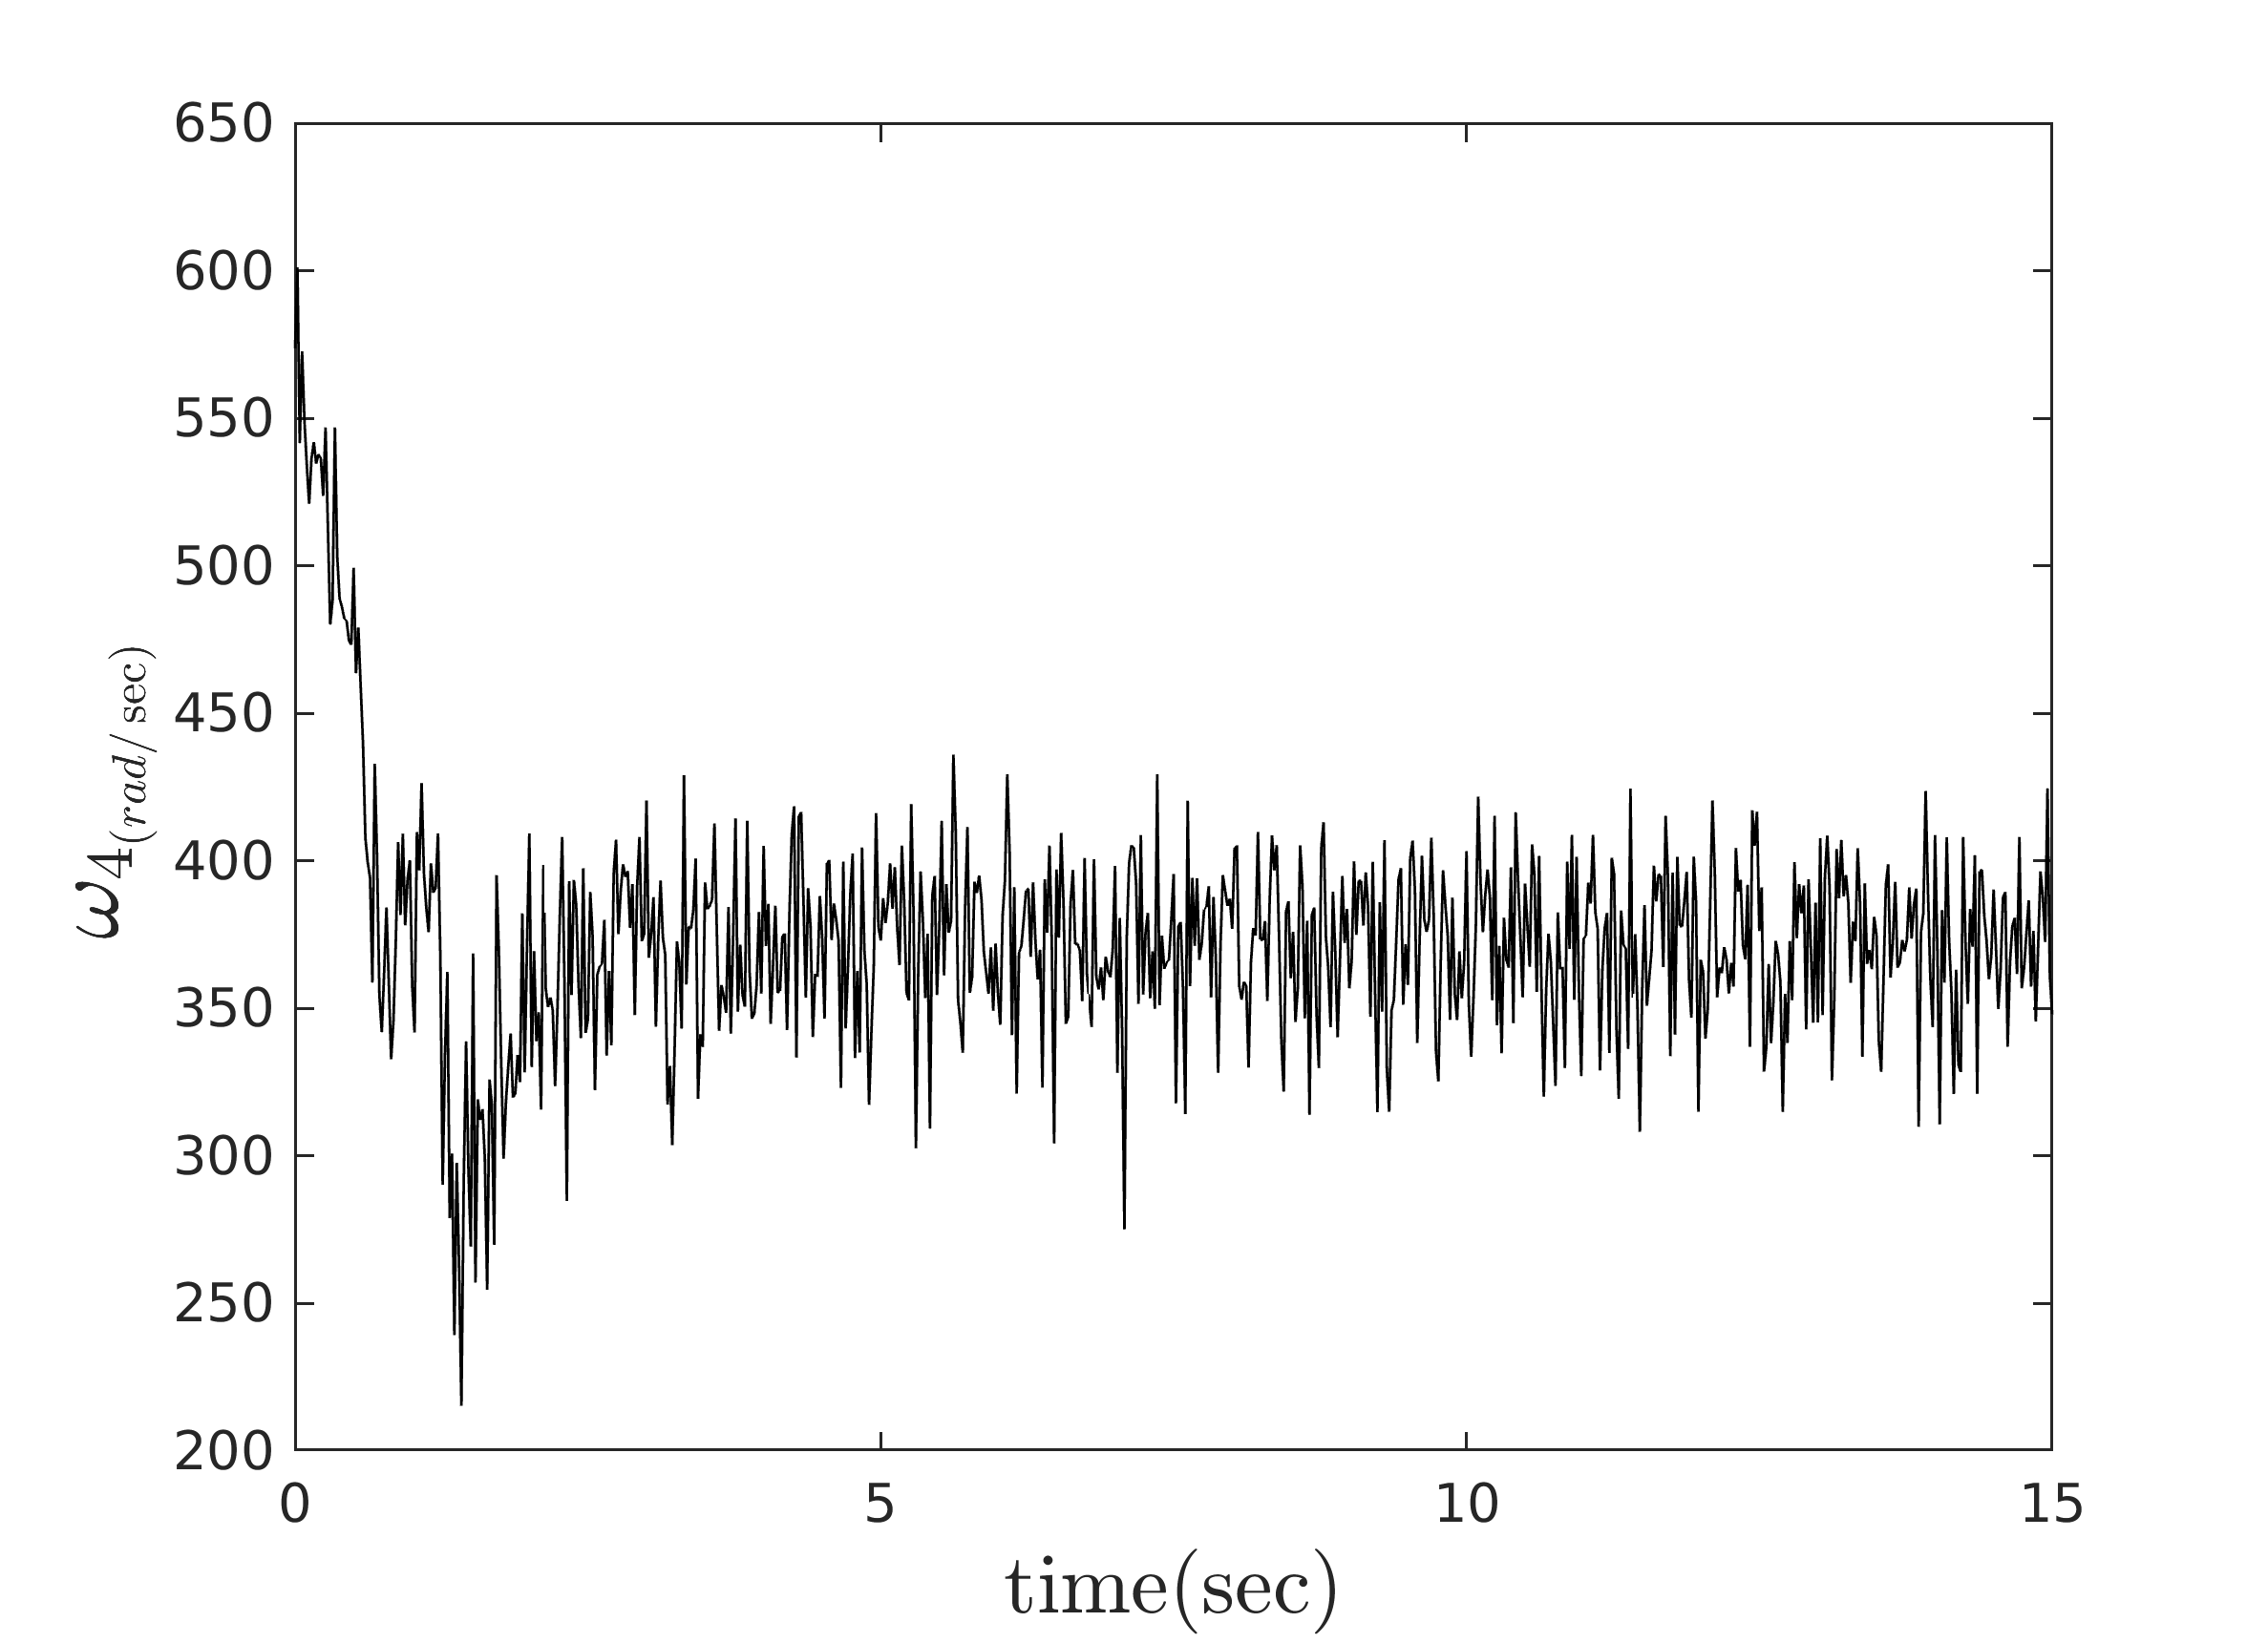
\includegraphics[width=.45\linewidth]{../Figures/MIL/LQIDG/3DOF/lqidg_roll_pitch_Omega_4.png}
	}
	\caption{‫‪فرمان کنترلی موتورها در کنترل زاویه رول، پیچ و یاو (تعقیب ورودی صفر)}
\end{figure}



%بر اساس خروجی شبیه‌سازی (شکل
%\ref{lqidg_roll_fig})
%،کانال رول در حضور کنترل‌کننده LQIDG در حدود پنج ثانیه و کانال پیچ در حدود هشت ثانیه به تعادل می‌رسد و خطای ماندگار آن در حدود صفر است.